\documentclass[11pt,conference,onecolumn]{IEEEtran}
\IEEEoverridecommandlockouts
% The preceding line is only needed to identify funding in the first footnote. If that is unneeded, please comment it out.
\usepackage[utf8]{inputenc}
\usepackage[T1]{fontenc}
\usepackage{amsthm}
\usepackage{amsmath,amssymb,amsfonts}
\usepackage{cite}
\usepackage{algorithmic}
\usepackage{multirow}
\usepackage{graphicx}
\usepackage{textcomp}
\usepackage{xcolor}
\usepackage{setspace}
\usepackage{verbatimbox}
\usepackage{thmtools}
\usepackage{float}
\usepackage{subcaption} % usado para figuras lado a lado
\usepackage[pdftex]{hyperref}

\declaretheoremstyle[spaceabove=6pt, spacebelow=6pt,headfont=\normalfont\bfseries,notefont=\mdseries, notebraces={(}{)},bodyfont=\normalfont,postheadspace=0.6em,
headpunct=:]{mystyle}
\declaretheorem[style=mystyle, name=Hypothesis, preheadhook={\renewcommand{\thehyp}{H\textsubscript{\arabic{hyp}}}}]{hyp}

\usepackage{cleveref}
\crefname{hyp}{hypothesis}{hypotheses}
\Crefname{hyp}{Hypothesis}{Hypotheses}

\def\BibTeX{{\rm B\kern-.05em{\sc i\kern-.025em b}\kern-.08em
    T\kern-.1667em\lower.7ex\hbox{E}\kern-.125emX}}
\begin{document}

\title{Sorting algorithms: how are they affected by memory faults?}

\author{\IEEEauthorblockN{Alexandro Vladno}
\IEEEauthorblockA{\textit{Centre for Informatics and Systems} \\
\textit{University of Coimbra}\\
Coimbra, Portugal \\
alexandro.vladno@gmail.com}
\and
\IEEEauthorblockN{Fabiano Papaiz}
\IEEEauthorblockA{\textit{Centre for Informatics and Systems} \\
\textit{University of Coimbra}\\
Coimbra, Portugal \\
fabianopapaiz@gmail.com}
\and
\IEEEauthorblockN{Leo Moreira Silva}
\IEEEauthorblockA{\textit{Centre of Informatics and Systems} \\
\textit{University of Coimbra}\\
Coimbra, Portugal \\
leo.moreira@me.com}
}

\maketitle

\begin{abstract}
This document is a model and instructions for \LaTeX.
This and the IEEEtran.cls file define the components of your paper [title, text, heads, etc.]. *CRITICAL: Do Not Use Symbols, Special Characters, Footnotes, 
or Math in Paper Title or Abstract.
\end{abstract}

\begin{IEEEkeywords}
component, formatting, style, styling, insert
\end{IEEEkeywords}

\onehalfspacing

\section{Introduction}
Technology is deeply introduced in people's quotidian supporting a massive number of tasks, for example: searching for a shared car, surfing on the web, sending a message to someone, automating the company's production or using the company's software. Nevertheless, most people don't know that devices are continually dealing with memory failures, faults and errors. These devices were made with large and inexpensive memories, which are also error-prone \cite{Finocchi2004}.

Software behavior may be affected by the problems mentioned before, especially those from memory. We have a memory fault when the correct value that should be stored in a memory location gets altered because of a soft failure. In particular, the content of a location can change unexpectedly, i.e., faults may happen at any time: real memory faults are indeed highly dynamic and unpredictable \cite{Hamdioui2003}.

In the beginning steps of software development, the designer has a general idea of the structure and functions. For each one of these, some algorithms will be produced or used. In the following stages, the outcome software (and its algorithms) will be tested and, then, delivered to the user. Different kinds of algorithms could be written or used in the software, and one of these is the sorting algorithms.

A good algorithm is that which gives satisfactory results for every range of data set. Sorting is a fundamental concept and important for solving other problems like is prerequisite for Binary Search. Sorting is often used in a large variety of critical applications and is a fundamental task that is used by most computers \cite{NitinArora}.

In this paper, we present a discussion about how these sorting algorithms, particularly Quicksort, Mergesort, Insertion Sort and Bubblesort, are affected by memory faults.

\section{Background}

In this section, we'll provide some definitions of memory faults and used sorting algorithms.

\subsection{Memory Faults}

Despite the title of this subsection, when the entire digital system (or software) is considered, there are three terms for computing fault and they have different meanings: failure, fault and error. 

A failure denotes an element's inability to perform its functions because of error in the element itself or its environment. A fault is an anomalous physical condition. Causes include design errors, manufacturing problems, damage, fatigue, or other deterioration. Faults resulting from design errors and external factors are especially difficult to model and protect against because their occurrences and effects are hard to predict. An error is a manifestation of a fault in a system, in which the logical state of an element differs from its intended value. A fault in a system does not necessarily result in an error. An error occurs for a particular system state and input when an incorrect next state and/or output results \cite{Nelson1990}.

\section{Experimental Setup}

In this section, we present the setup of this study. We first state our problem, then define the independent and dependent variables. After that, we show the hypothesis and describe our dataset, showing all its characteristics.

\subsection{Problem Statement}

As introduced in the first section of this paper, sorting is a fundamental concept and essential for solving other problems. The content of memory location can change unexpectedly, i.e., faults may happen at any time. Considering this, the main objective of this work is to design experiments to answer the following question: \textit{How are sorting algorithms affected by memory faults?}

\subsection{Variables}

For this experimental study, we assume that the independent and dependent variables are as shown in Table \ref{table-independent-variables} and Table \ref{table-dependent-variables} below:

\begin{table}[H]
    \caption{Independent variables.}
    \begin{center}
    \begin{tabular}{|l|l|}
    \hline
    \textbf{Variable} & \textbf{Description} \\
    \hline
    Probability of failure & Probability of a fault to occur \\
    \hline
    Array size & Size of the array of integers to be sorted \\
    \hline
    Sorting algorithm & Algorithm used to sort the array \\
    \hline
    \end{tabular}
    \label{table-independent-variables}
    \end{center}
\end{table}

\begin{table}[H]
    \caption{Dependent variables.}
    \begin{center}
    \begin{tabular}{|l|l|}
    \hline
    \textbf{Variable} & \textbf{Description} \\
    \hline
    Largest subarray size & Size of the largest sorted subarray produced under the memory fault \\
    \hline
    Percentage of largest subarray size & Percentage of \textit{largest subarray size} related to \textit{array size} independent variable \\
    \hline
    Unordered elements quantity & Quantity of elements out of position after sorting algorithm execution. Adapted of the \\ & \textit{k-unordered sequence} measure of disorder defined in \cite{Ferraro-Petrillo2009} \\
    \hline
    Percentage of unordered elements quantity & Percentage of \textit{unordered elements quantity} related to \textit{array size} independent variable \\
    \hline
    \end{tabular}
    \label{table-dependent-variables}
    \end{center}
\end{table}

\subsection{Hypothesis}

The set of hypothesis defined to test and draw some conclusions about this experiment are listed below. The confidence degree defined for hypothesis testing was 95\% ($\alpha = 0.05$ and $\alpha - 1 = 0.95$).

\begin{itemize}
    \item \textbf{Hypothesis 1:} For a given probability of failure and array size, tested algorithms will produce a different percentage of unordered elements quantity.
    \item \textbf{Hypothesis 2:} For a given probability of failure and array size, tested algorithms will produce a different percentage of the largest subarray size.
    \item \textbf{Hypothesis 3:} For each algorithm, the array size and probability of failure have a significative impact on the percentage of unordered elements quantity.
    \item \textbf{Hypothesis 4:} For each algorithm, the array size and probability of failure have a significative impact on the percentage of the largest subarray size.
\end{itemize}

\subsection{Dataset}

To conduct the proposed study, we define the values of the independent variables, as shown in Table \ref{table-independent-variables-values}:

\begin{table}[H]
    \caption{Values of the independent variables.}
    \begin{center}
    \begin{tabular}{|c|c|}
    \hline
    \textbf{Variable} & \textbf{Values} \\
    \hline
    Probability of failure & 1\%, 2\% and 5\% \\
    \hline
    Array size & 100, 1000 and 10000 \\
    \hline
    Sorting algorithm & Bubblesort, Quicksort, Mergesort and Insertionsort \\
    \hline
    \end{tabular}
    \label{table-independent-variables-values}
    \end{center}
\end{table}

Based on these variables, we ran an existing script \textit{gen.py} to produce input files. We define that our sample was composed by 30 input files for a given combination of the probability of failure and array size. So, considering this, we ran 30 times for each combination of these independent variables, producing 30 inputs, totalizing 270 files. Figure \ref{fig-input-file-example} shows an example of produced input files:

\begin{verbbox}[\mbox{}]
0.01 100 9 48 37 6 26 7 24 44 17 50 48 30 49 33 22 13 42 29 39 13 19 13 9 28 
34 1 33 27 14 45 48 40 11 17 6 50 9 44 20 16 37 45 23 14 38 29 10 49 44 46 35
45 15 2 22 1 46 40 8 48 23 23 32 35 3 15 8 36 17 24 27 48 28 5 28 50 44 4 25 
6 9 1 11 44 26 50 44 12 7 20 30 20 37 20 6 8 13 15 20 49
\end{verbbox}

\begin{figure}[H]
    \centering
    \fbox{
    \theverbbox
    }
    \caption{Example of input file.}
    \label{fig-input-file-example}
\end{figure}

The input data shown in the Figure \ref{fig-input-file-example} is divided as follows:

\begin{itemize}
    \item \textit{Probability of Failure}: the first number of the sequence (\texttt{0.01}) is the probability of memory failure when sorting;
    \item \textit{Sequence size}: the second number (\texttt{100}) means the size of the integers sequence used by sorting;
    \item \textit{Sequence}: the rest of the numbers represents a list of \textit{n} positive integers that will be sorted.
\end{itemize}

With this input data, we ran, for each one of these, all four algorithms considered in this study. The sorting algorithms used already existed. For example, using all 270 input files, we ran bubblesort, creating 270 output files, and so on for the other algorithms. At the end of executions, we get a total of 1080 output files. An output file looks like shown in Figure \ref{fig-output-file-example}:

\begin{verbbox}[\mbox{}]
[1]  9 48 37 6 26 7 24 44 17 50 48 30 49 33 22 13 42 29 39 13 19 13 9 28 34 1
33 27 14 45 48 40 11 17 6 50 9 44 20 16 37 45 23 14 38 29 10 49 44 46 35 45  
15 2 22 1 46 40 8 48 23 23 32 35 3 15 8 36 17 24 27 48 28 5 28 50 44 4 25 6 9
1 11 44 26 50 44 12 7 20 30 20 37 20 6 8 13 15 20 49
[2]  1 1 1 2 3 4 5 6 6 6 6 7 7 8 8 8 9 9 9 9 10 11 11 12 13 13 13 13 14 14 15 
15 15 16 17 17 17 19 20 20 20 20 22 22 23 23 23 24 24 25 26 26 27 27 28 28 28 
29 29 30 30 32 33 33 34 35 35 36 37 37 37 38 39 40 40 42 44 44 44 44 44 44 20 
45 45 45 46 46 48 48 48 48 48 49 49 50 49 50 50 50
[3]  1 1 1 2 3 4 5 6 6 6 6 7 7 8 8 8 9 9 9 9 10 11 11 12 13 13 13 13 14 14 15 
15 15 16 17 17 17 19 20 20 20 20 20 22 22 23 23 23 24 24 25 26 26 27 27 28 28 
28 29 29 30 30 32 33 33 34 35 35 36 37 37 37 38 39 40 40 42 44 44 44 44 44 44 
45 45 45 46 46 48 48 48 48 48 49 49 49 50 50 50 50
[4]  82
\end{verbbox}
    
\begin{figure}[H]
    \centering
    \fbox{
    \theverbbox
    }
    \caption{Example of output file.}
    \label{fig-output-file-example}
\end{figure}

The output file gives four essential data, as enumerated below:
\begin{itemize}
    \item \textit{1)} the original sequence of integers contained in the input file;
    \item \textit{2)} the sequence processed by the sorting algorithm under the memory fault model;
    \item \textit{3)} the sequence sorted correctly;
    \item \textit{4)} the size of the largest sorted subsequence in item \textit{2}. This number can be interpreted as a quality measure. As higher, most successful was the sorting operation.
\end{itemize}

After generating the dataset, we developed a Python program that reads the 1080 output files and produces a single CSV file (first lines showed in Figure \ref{fig-output-csv-file-example}). This file contains the columns listed below and was used to perform the exploratory data analysis and to run the statistical tests.
\begin{itemize}
    \item \textit{sorting\_algorithm}: the algorithm used to sort the array;
    \item \textit{probability\_of\_failure}: the probability of failure used when sorting;
    \item \textit{array\_size}: the size of the sorted array;
    \item \textit{largest\_subarray\_size}: the largest sorted subarray after sorting;
    \item \textit{unordered\_elements\_quantity}: quantity of unordered sequence elements after sorting.
    \item \textit{perc\_unordered\_elements\_quantity}: percentage of unordered elements after sorting related to original array;
    \item \textit{perc\_largest\_subarray\_size}: percentage of largest sorted subarray after sorting related to original array.
\end{itemize}

\begin{verbbox}[\mbox{}]
sorting_algorithm;probability_of_failure;array_size;largest_subarray_size;
unordered_elements_quantity;perc_unordered_elements_quantity;
perc_largest_subarray_size
quick;0.01;100;35;4;4.00;35.00
quick;0.01;100;36;8;8.00;36.00
quick;0.01;100;31;5;5.00;31.00
quick;0.01;100;20;6;6.00;20.00
quick;0.01;100;31;5;5.00;31.00
\end{verbbox}
        
\begin{figure}[H]
    \centering
    \fbox{
    \theverbbox
    }
    \caption{Example of output CSV file.}
    \label{fig-output-csv-file-example}
\end{figure}

We use Python libraries to make data analysis and plot graphs. These libraries were:
\begin{itemize}
    \item \textit{Pandas\footnote{https://pandas.pydata.org}}: open source library providing data structures and data analysis tools;
    \item \textit{NumPy\footnote{https://numpy.org}}: library for scientific computing with Python;
    \item \textit{SciPy\footnote{https://www.scipy.org}}: ecosystem of open-source software for mathematics, science, and engineering;
    \item \textit{StatsModels\footnote{https://www.statsmodels.org}}: module that provides classes and functions for the estimation of many different statistical models, as well as for conducting statistical tests, and statistical data exploration;
    \item \textit{Matplotlib\footnote{https://matplotlib.org}}: plotting library;
    \item \textit{Seaborn\footnote{https://seaborn.pydata.org}}: data visualization library based on matplotlib.
\end{itemize}

\section{Data Analysis}

In this section, we present our results after the execution of sorting algorithms over the input files. We analyzed only two of the four dependent variables, which were \textit{percentage of the largest subarray size (\%LSS)} and \textit{percentage of unordered elements quantity (\%UEQ)}. These variables, because they are a percentage value, already were normalized (i.e., the same order of magnitude) related to dependent variable \textit{array size}.

\subsection{Exploratory Data Analysis (EDA)}

Firstly, we performed an analysis of the distribution of the dependent variables \%LSS and \%UEQ. To help in this task, we produced histograms, boxplot graphs, tables containing data about mean, median, standard deviation, and the minimum and maximum values.

The following Figures \ref{fig-histogram-boxplot-bubble-001100}, \ref{fig-histogram-boxplot-insertion-001100}, \ref{fig-histogram-boxplot-merge-00510000} and \ref{fig-histogram-boxplot-quick-00510000} illustrates examples of histograms and boxplot graphs for each combination of \textit{Algorithm X Probability of Failure X Array Size}. In each of those figures, the graphs were exhibited over the dependent variables \%LSS and \%UEQ.  In the histogram, the red vertical line means the mean, and the blue vertical line means the median. On the other hand, in the boxplot, the red horizontal line means the mean, and the blue horizontal line means the median.

\begin{figure}[H]
    \centering
    \frame{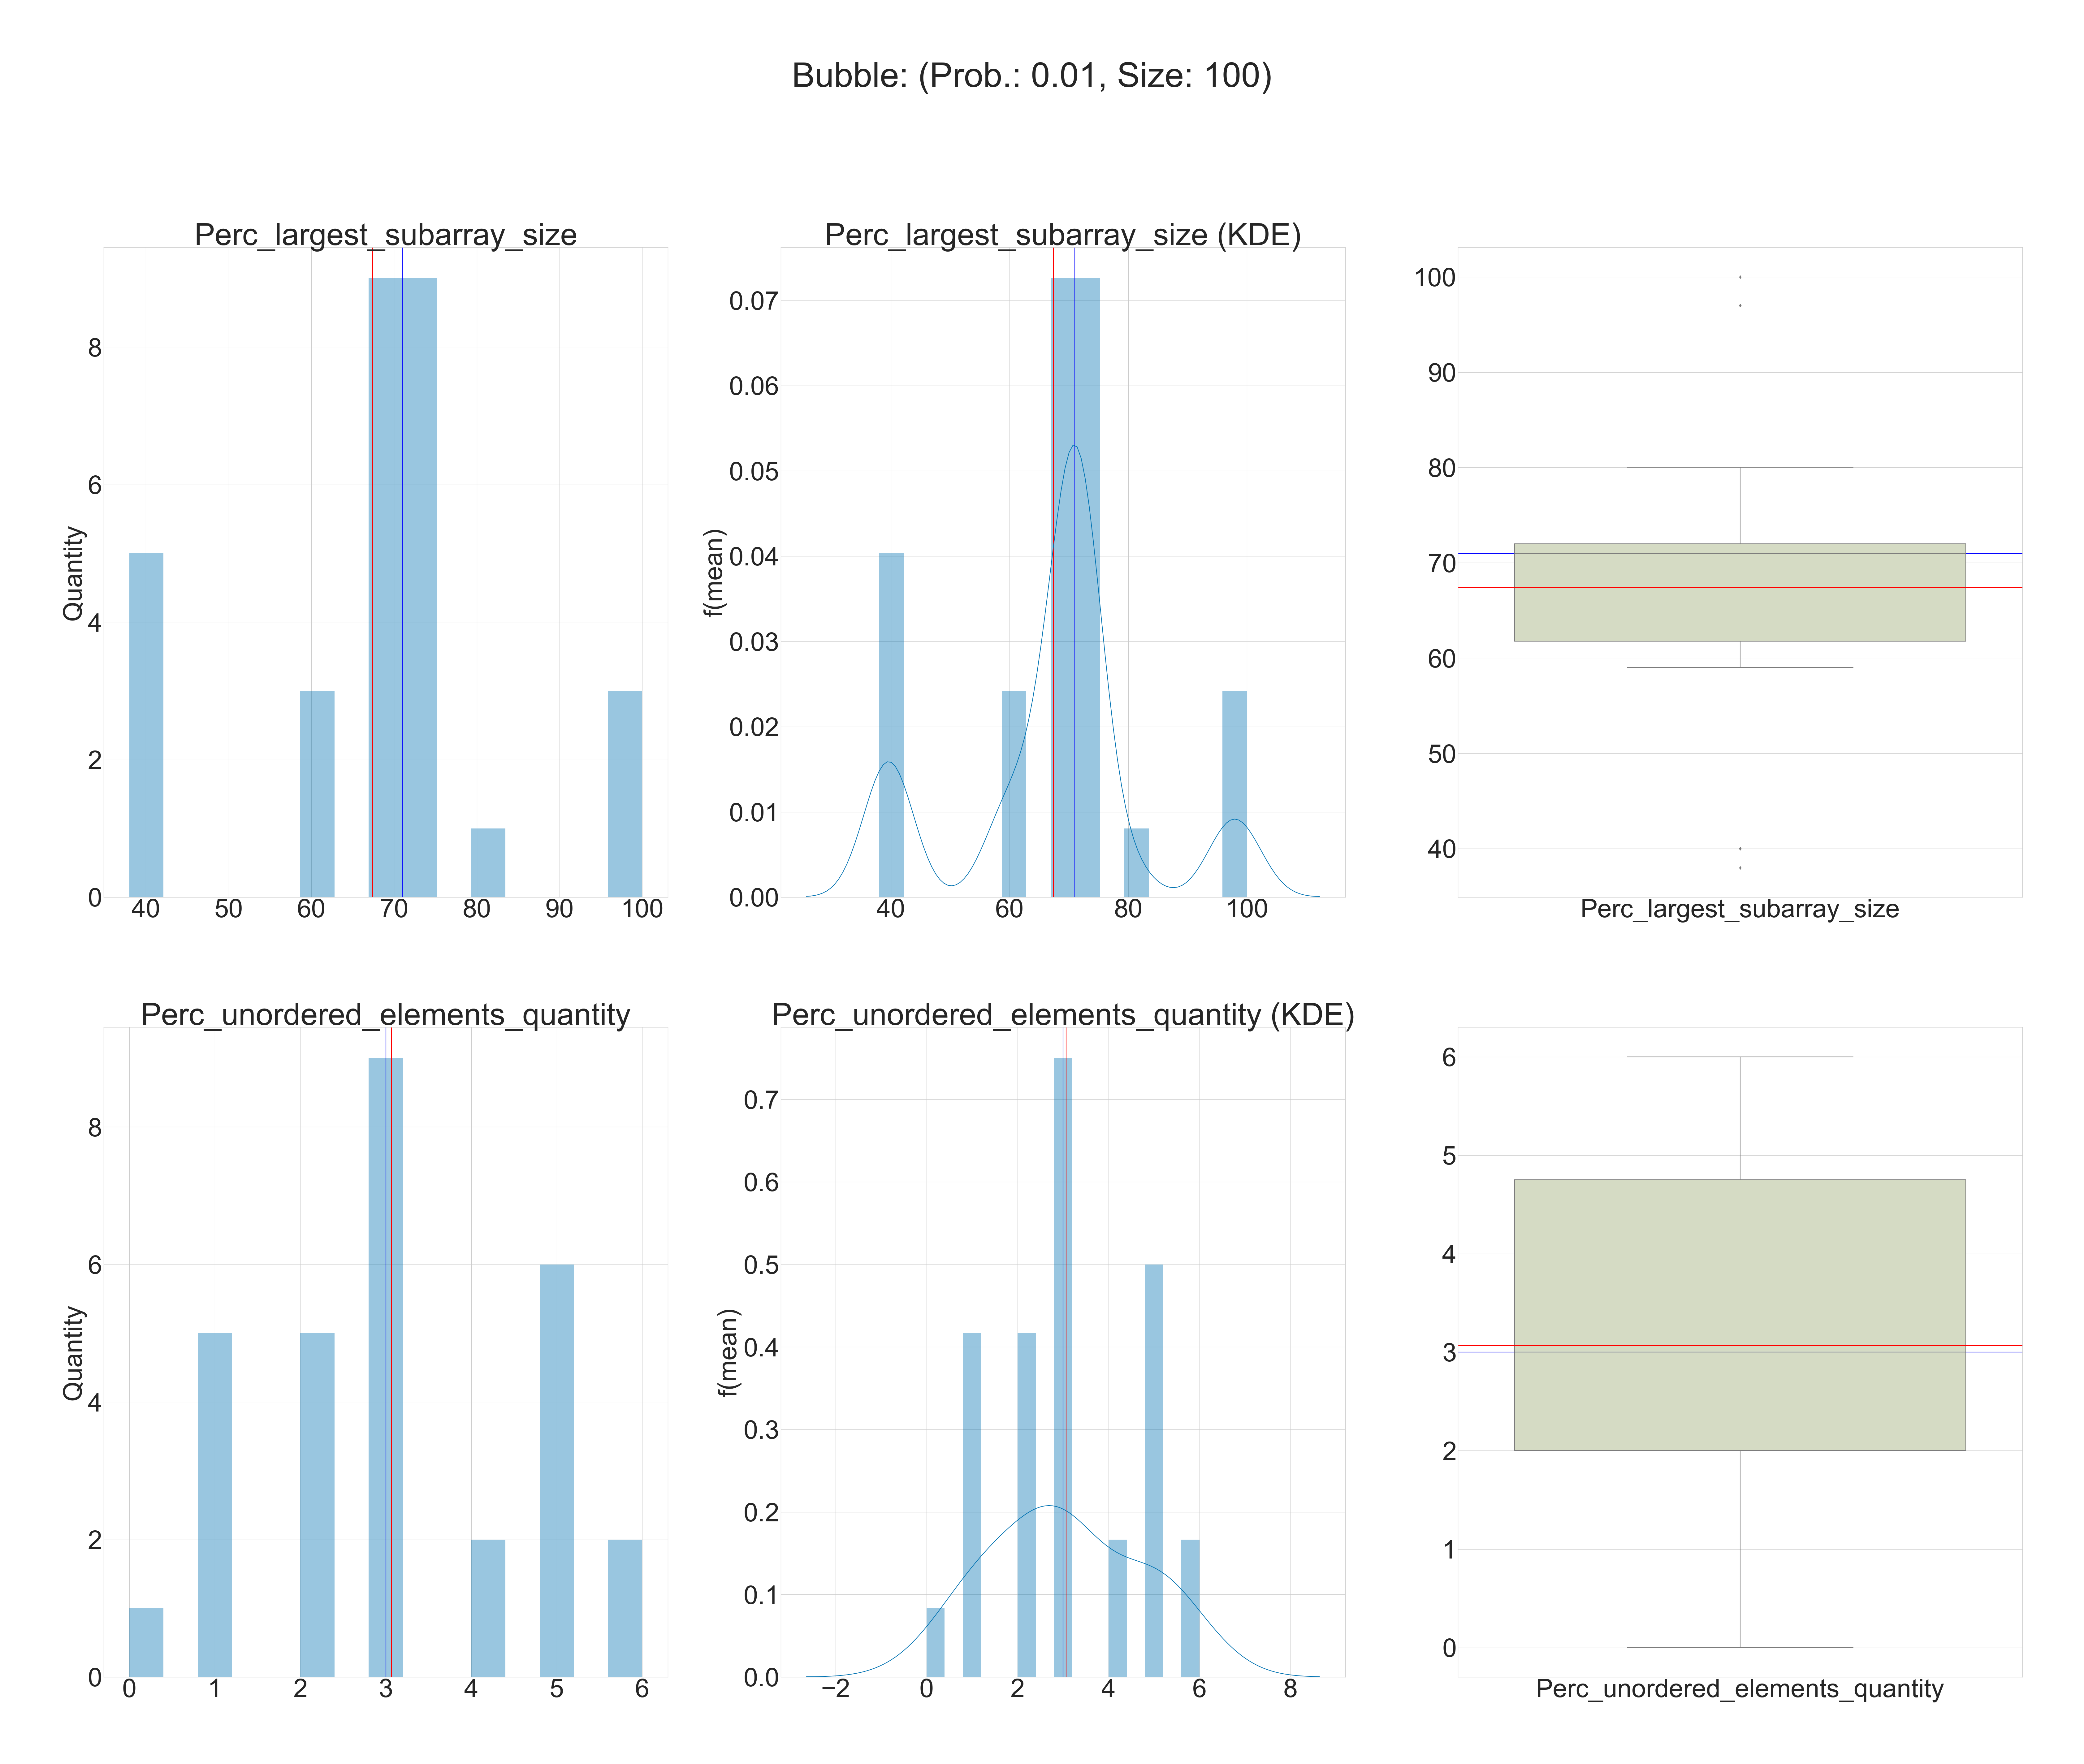
\includegraphics[scale=0.105]{figures/0_01_100_Bubble.png}}
    \caption{Histograms and Boxplot for Bubblesort, with \textit{probability of failure} of 0.01 and \textit{array size} of 100.}
    \label{fig-histogram-boxplot-bubble-001100}
\end{figure}

Based on Figures \ref{fig-histogram-boxplot-bubble-001100}, \ref{fig-histogram-boxplot-insertion-001100}, \ref{fig-histogram-boxplot-merge-00510000} and \ref{fig-histogram-boxplot-quick-00510000}, the following Tables \ref{tab-distribution-depentent-variable-ueq} and \ref{tab-distribution-depentent-variable-lss} illustrates the information about the dependent variables (\%LSS and \%UEQ) distribution.

\begin{table}[H]
    \caption{Table Type Styles}
    \begin{center}
    \begin{tabular}{|c|c|c|c|c|c|c|c|}
    \hline
    \textbf{Prob. of Failure} & \textbf{Array Size} & \textbf{Algorithm} & \multicolumn{5}{|c|}{\textbf{Percentage of unordered elements quantity (\%UEQ)}} \\
    \cline{4-8} 
    & & & \textbf{\textit{Mean}}& \textbf{\textit{Median}} & \textbf{\textit{Std. Deviation}} & \textbf{\textit{Minimum}} & \textbf{\textit{Maximum}} \\
    \hline
    0.01 & 100 & bubble & 3.07 & 3.0 & 1.64 & 0.0 & 6.0 \\
    \hline
    0.01 & 100 & insertion & 10.87 & 11.0 & 1.59 & 8.0 & 14.0 \\
    \hline
    0.05 & 10000 & merge & 28.32 & 28.34 & 0.31 & 27.69 & 28.86 \\
    \hline
    0.05 & 10000 & quick & 19.56 & 19.58 & 0.26 & 18.95 & 20.07 \\
    \hline
    \end{tabular}
    \label{tab-distribution-depentent-variable-ueq}
    \end{center}
\end{table}

\begin{figure}[H]
    \centering
    \frame{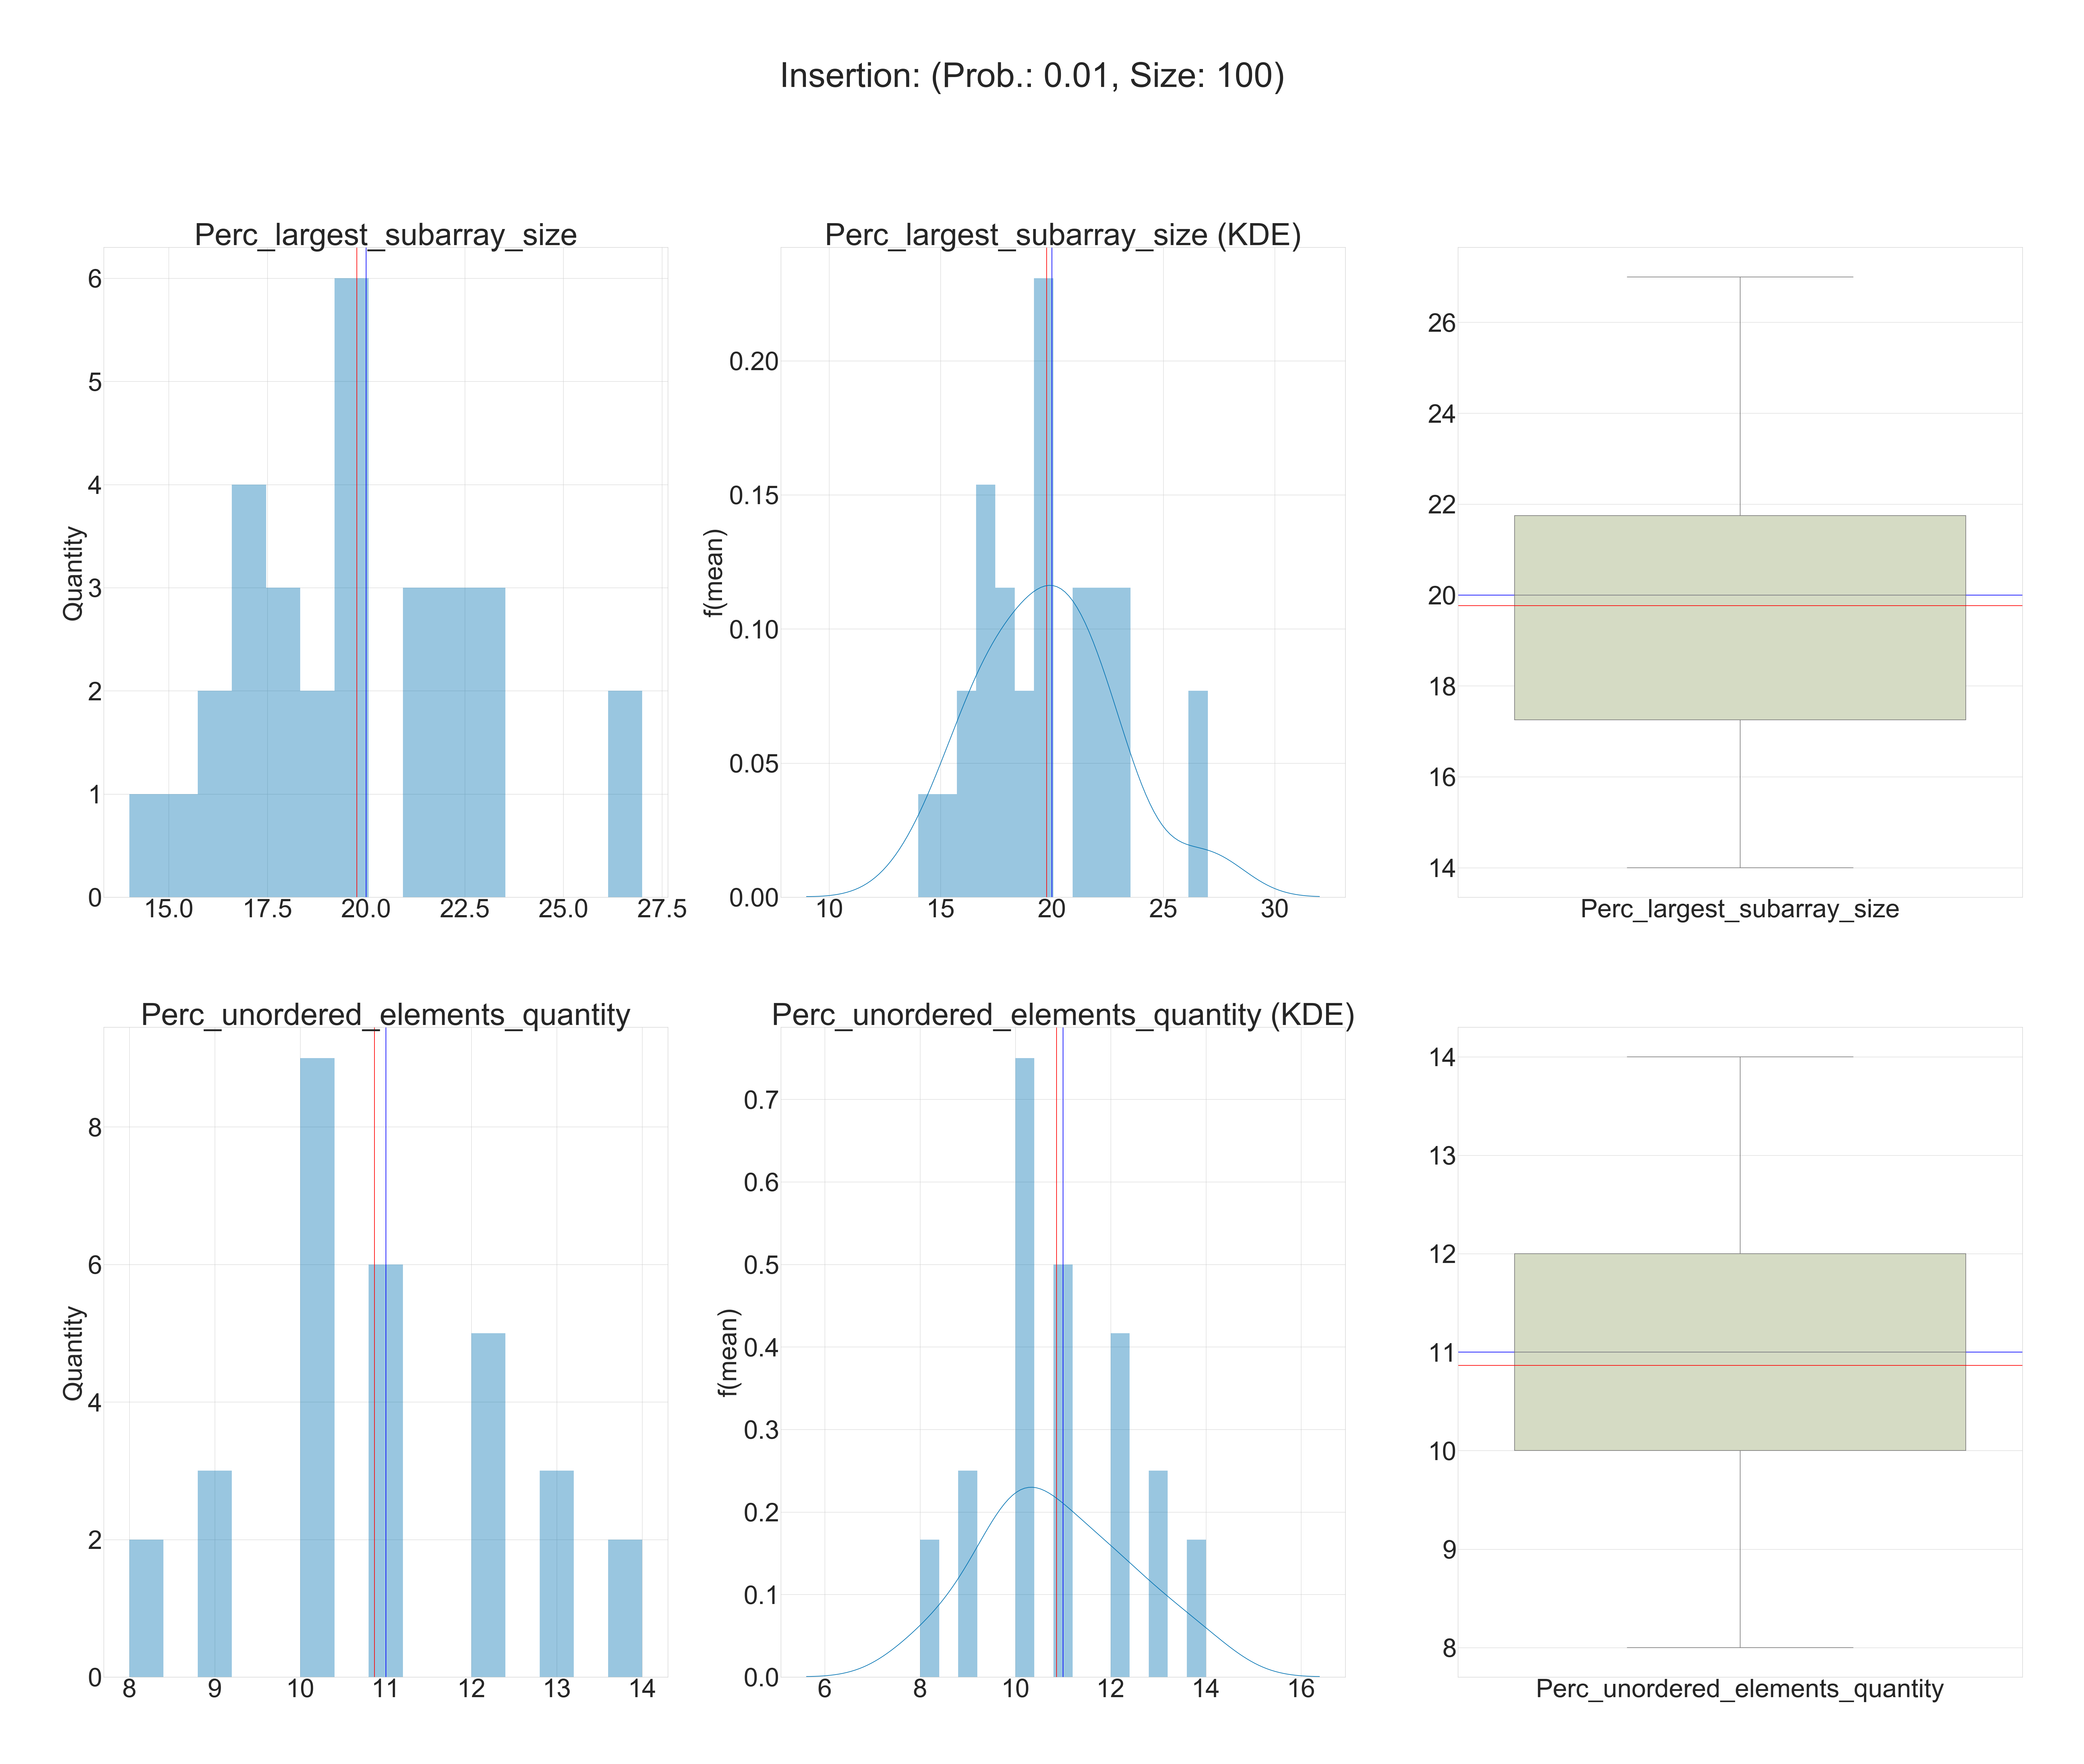
\includegraphics[scale=0.105]{figures/0_01_100_Insertion.png}}
    \caption{Histograms and Boxplot for Insertion sort, with \textit{probability of failure} of 0.01 and \textit{array size} of 100.}
    \label{fig-histogram-boxplot-insertion-001100}
\end{figure}

\begin{table}[H]
    \caption{Table Type Styles}
    \begin{center}
    \begin{tabular}{|c|c|c|c|c|c|c|c|}
    \hline
    \textbf{Prob. of Failure} & \textbf{Array Size} & \textbf{Algorithm} & \multicolumn{5}{|c|}{\textbf{Percentage of largest subarray size (\%LSS)}} \\
    \cline{4-8} 
    & & & \textbf{\textit{Mean}}& \textbf{\textit{Median}} & \textbf{\textit{Std. Deviation}} & \textbf{\textit{Minimum}} & \textbf{\textit{Maximum}} \\
    \hline
    0.01 & 100 & bubble & 67.4 & 71.0 & 15.84 & 38.0 & 100.0 \\
    \hline
    0.01 & 100 & insertion & 19.77 & 20.0 & 3.11 & 14.0 & 27.0 \\
    \hline
    0.05 & 10000 & merge & 0.19 & 0.2 & 0.03 & 0.15 & 28.86 \\
    \hline
    0.05 & 10000 & quick & 0.3 & 0.3 & 0.03 & 0.23 & 0.34 \\
    \hline
    \end{tabular}
    \label{tab-distribution-depentent-variable-lss}
    \end{center}
\end{table}

\begin{figure}[H]
    \centering
    \frame{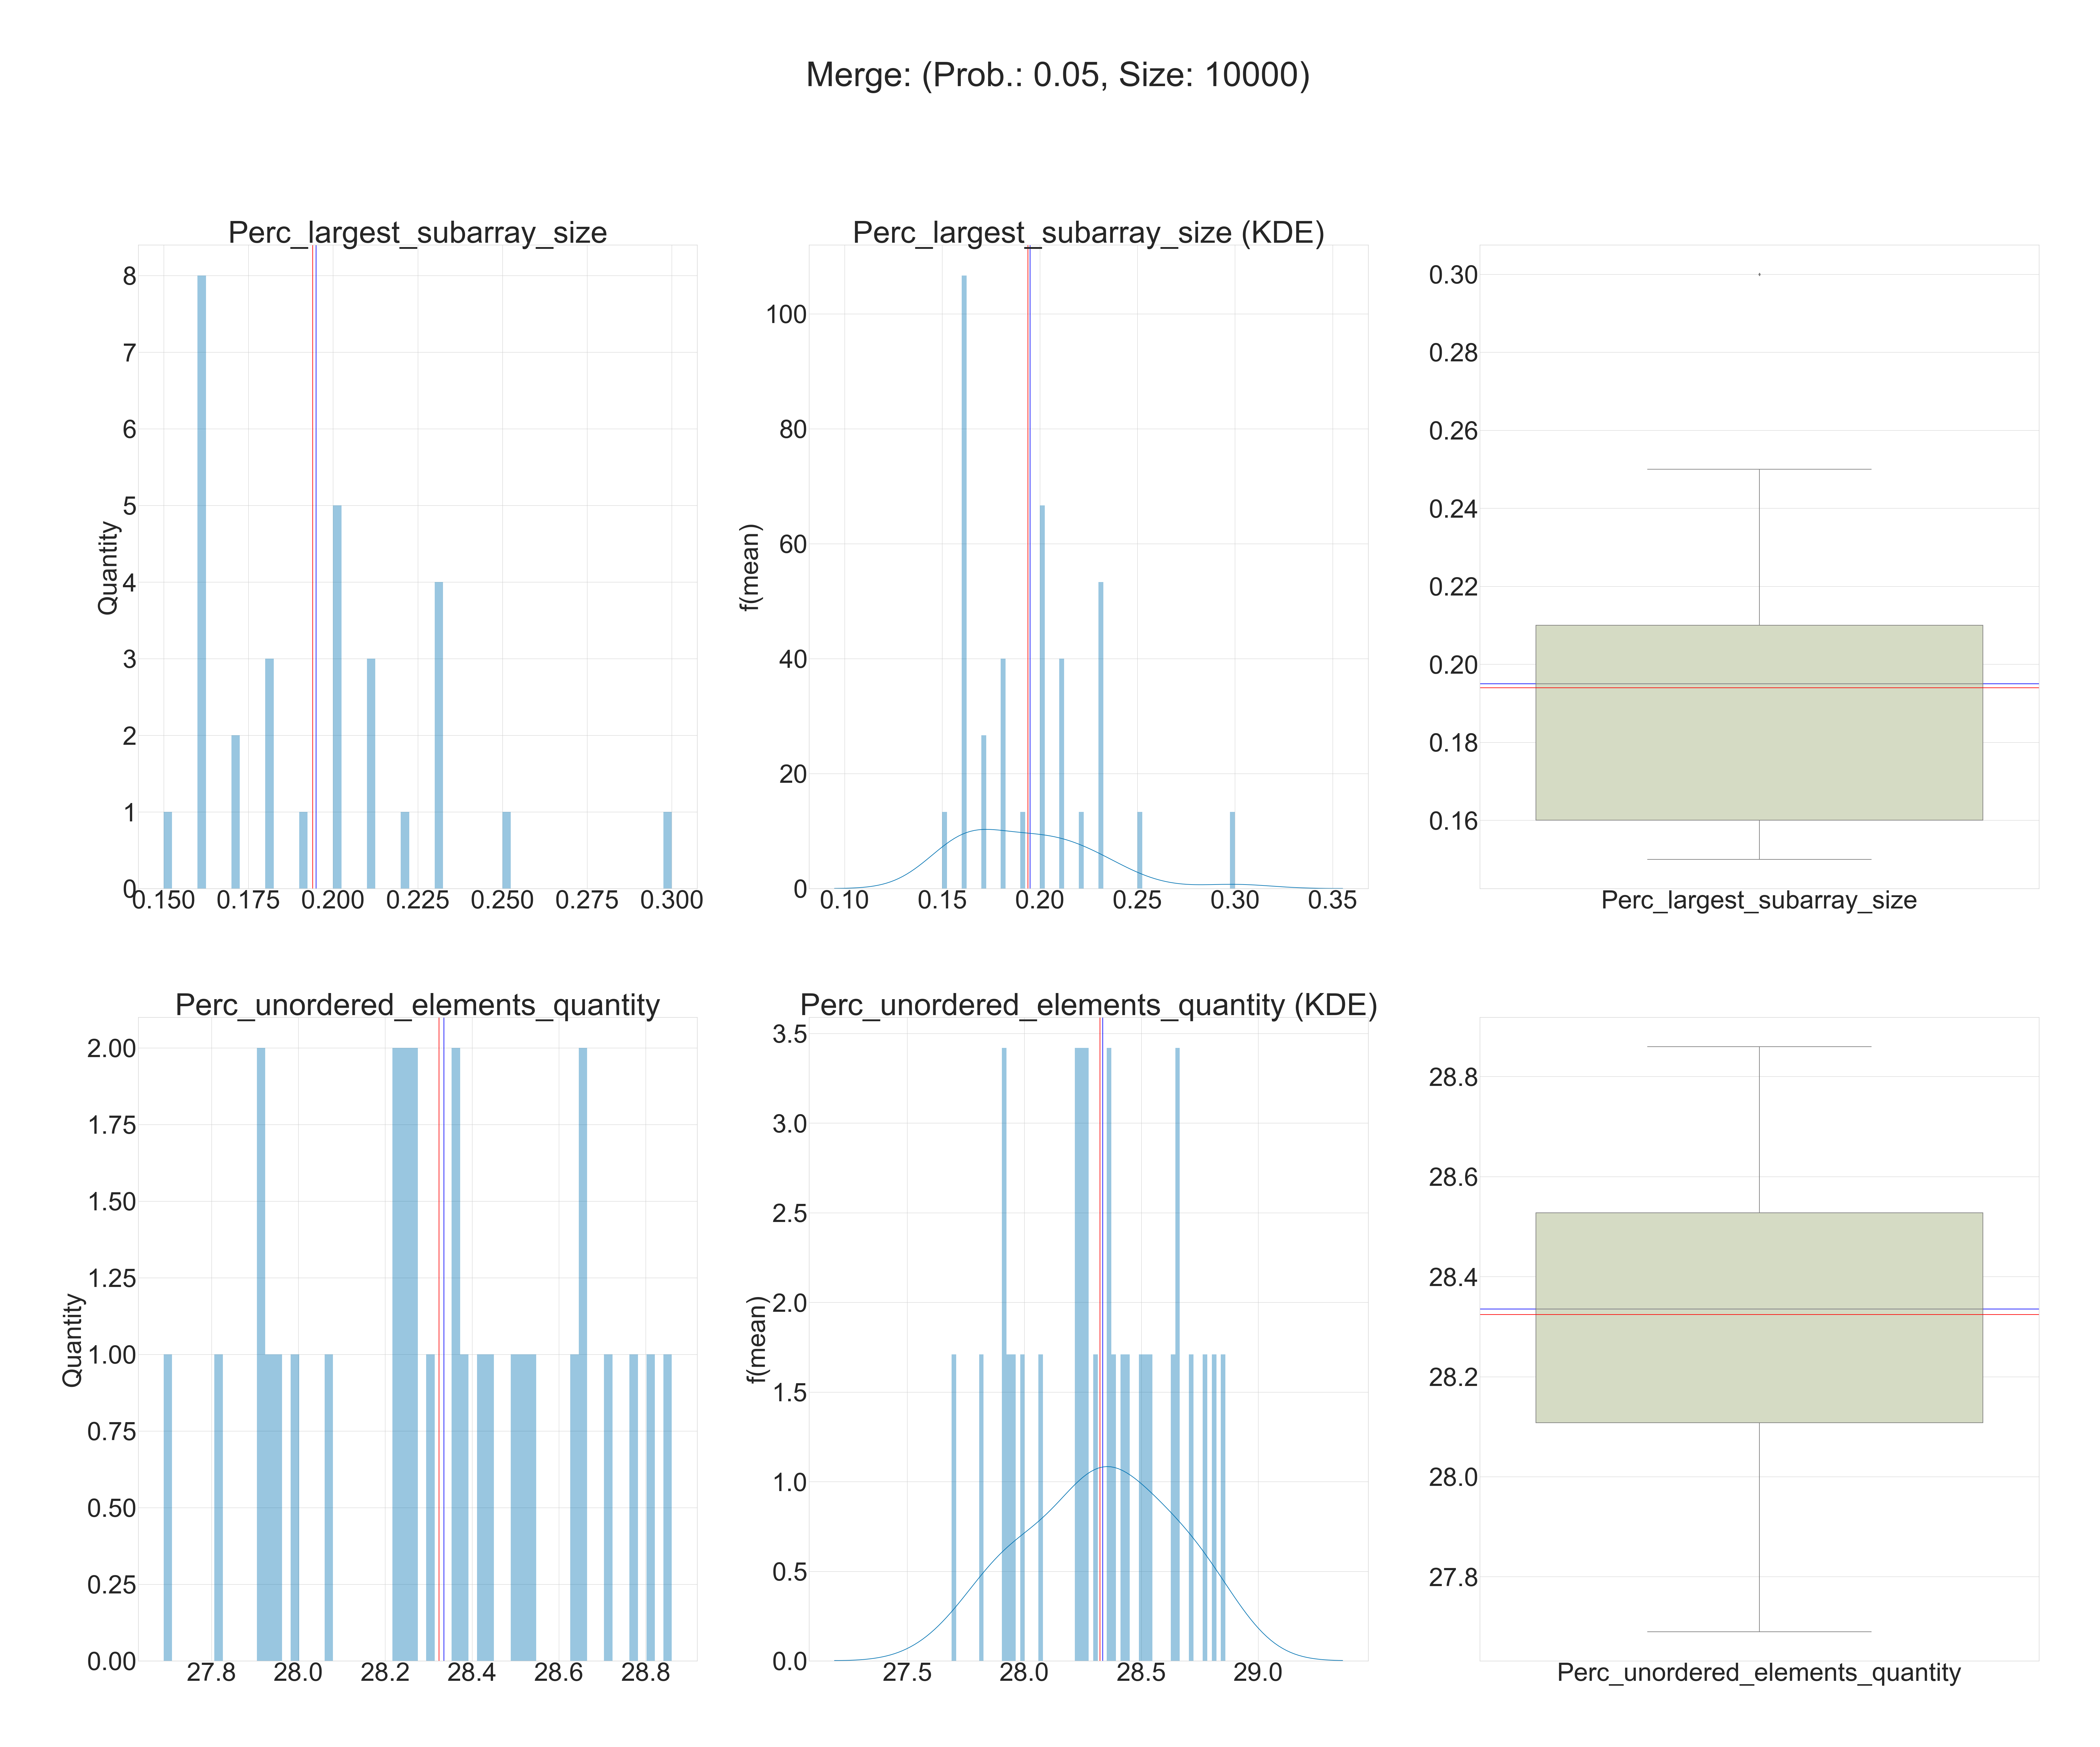
\includegraphics[scale=0.105]{figures/0_05_10000_Merge.png}}
    \caption{Histograms and Boxplot for Mergesort, with \textit{probability of failure} of 0.05 and \textit{array size} of 10000.}
    \label{fig-histogram-boxplot-merge-00510000}
\end{figure}

\begin{figure}[H]
    \centering
    \frame{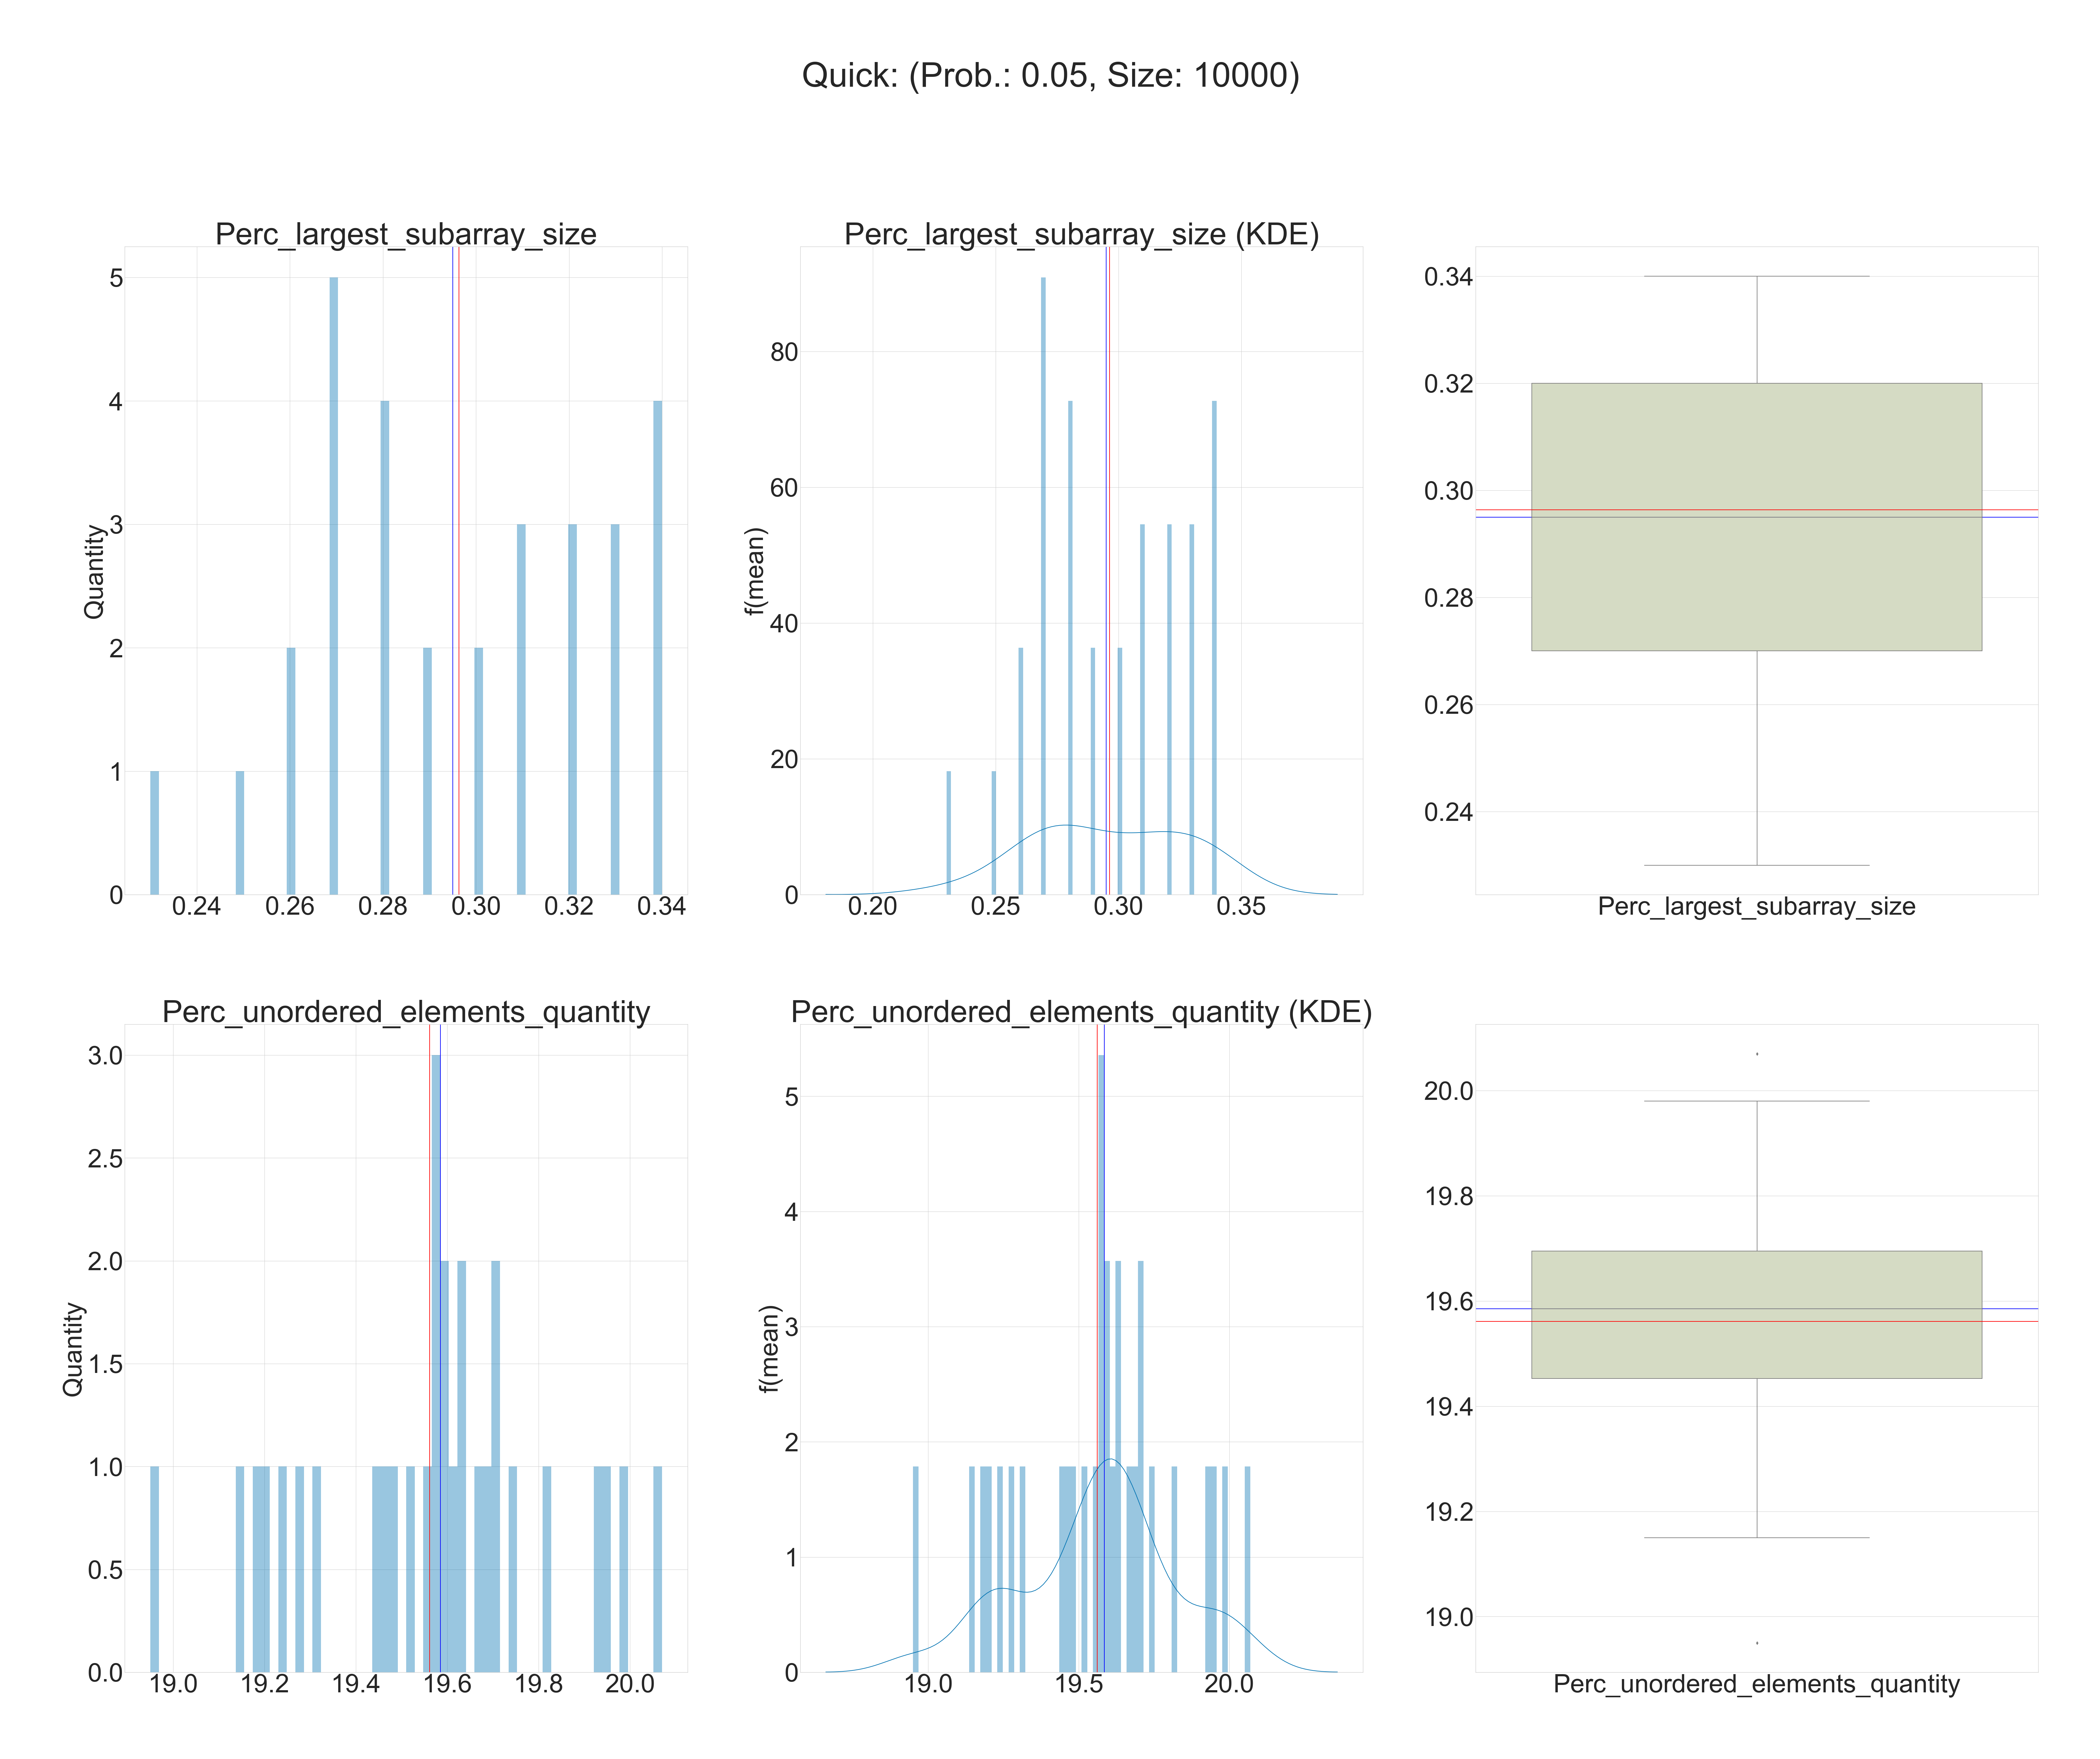
\includegraphics[scale=0.105]{figures/0_05_10000_Quick.png}}
    \caption{Histograms and Boxplot for Quicksort, with \textit{probability of failure} of 0.05 and \textit{array size} of 10000.}
    \label{fig-histogram-boxplot-quick-00510000}
\end{figure}

We produced graphs with the same data showed in Tables \ref{tab-distribution-depentent-variable-ueq} and \ref{tab-distribution-depentent-variable-lss}. Figure \ref{fig-distribution-all-algorithms-001-all-sizes} shows an example of these graphs. On it, we illustrate on the top-left graph that, considering the mean, bubblesort produces fewer unordered elements related to the total than other algorithms.

\begin{figure}[H]
    \centering
    \frame{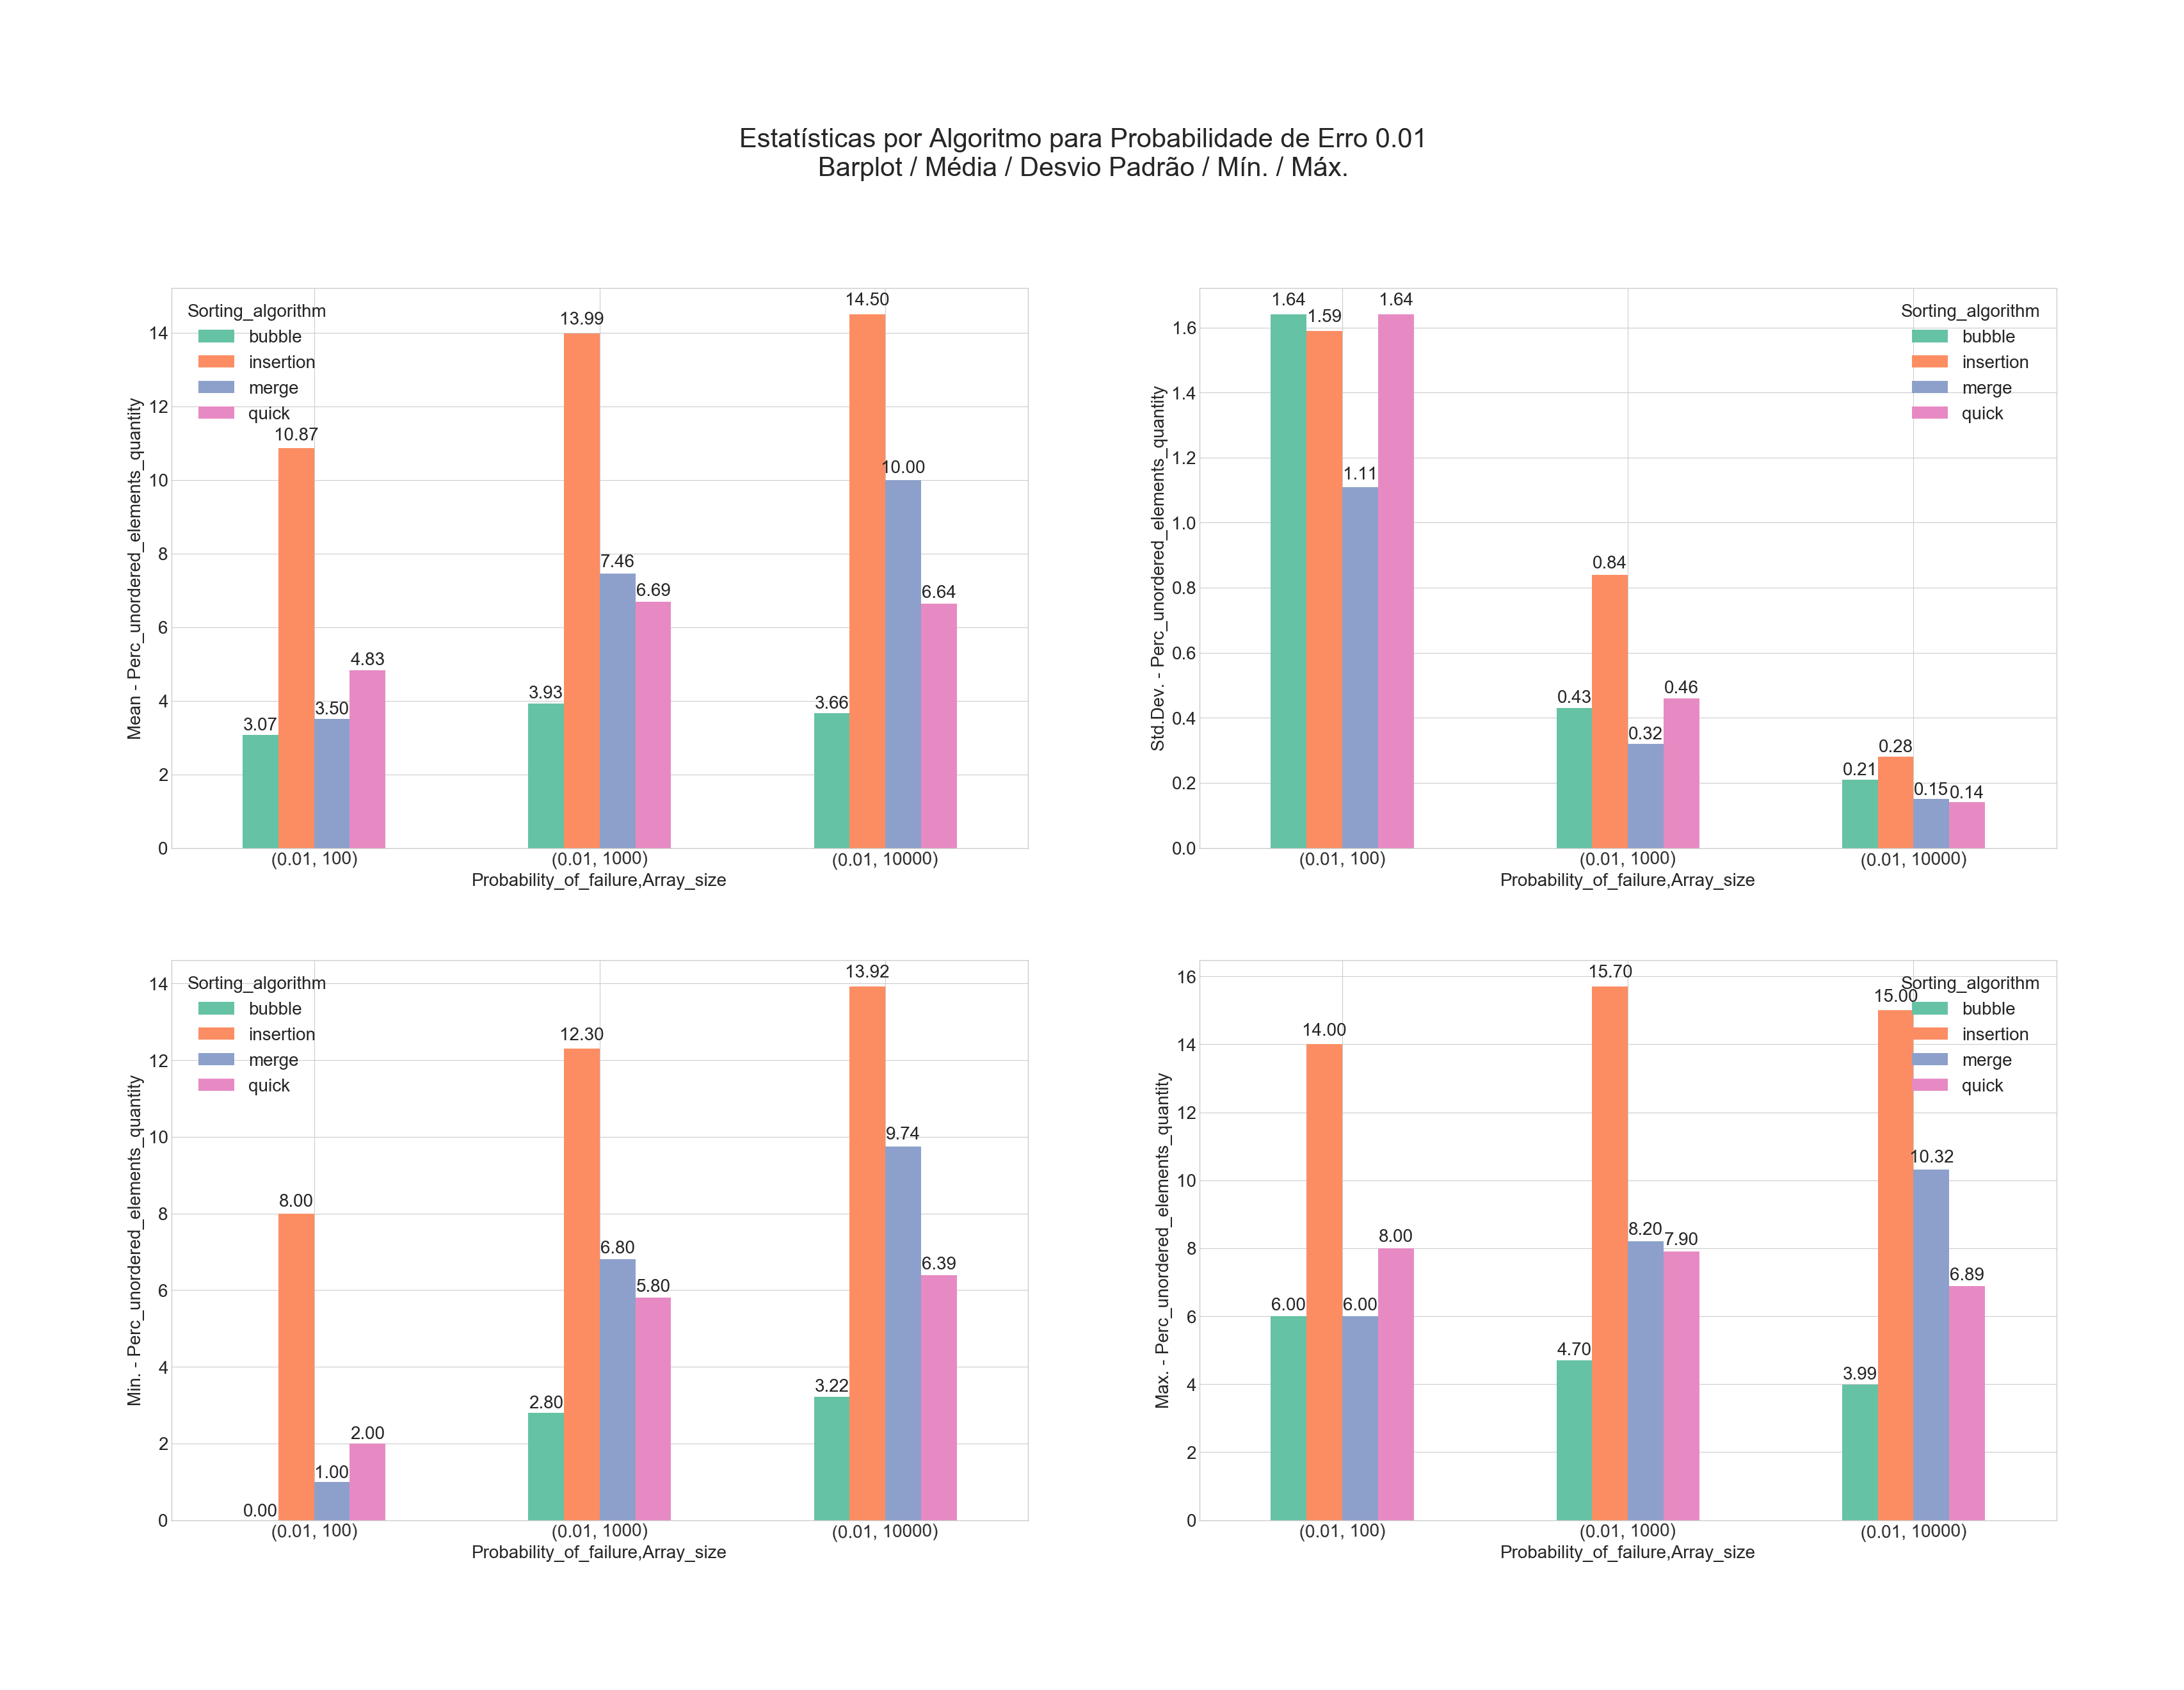
\includegraphics[scale=0.20]{figures/Estatisticas_por_Algoritmo_Prob_001.png}}
    \caption{Distribution data with \textit{probability of failure} of 0.01, all algorithms and \textit{array sizes}.}
    \label{fig-distribution-all-algorithms-001-all-sizes}
\end{figure}

\subsection{Dependent Variables Normality}

An essential step to continue the analysis is to verify if dependent variables have a normal distribution. In this work, we produced the Q-Q plot to analyze the normality visually. We also ran the Shapiro-Wilk \cite{shapiro1965analysis} test to confirm if they follow a normal distribution or not.

After the Shapiro-Wilk test, we determine that only the dependent variable \%UEQ (\textit{percentage of unordered elements quantity}) has a normal distribution related to mean for all algorithms. This situation occurred considering all possible combinations between independent variables: \textit{sorting algorithm}, \textit{probability of failure} and \textit{array size}.

Based on these results, we choose to test just the hypothesis associated with the dependent variable \%UEQ. We made use of the ANOVA method to test the hypothesis, and this method is premised the normal distribution of variables values.

Tables \ref{table-shapiro-test-lss-001-100} and \ref{table-shapiro-test-ueq-001-100} shows examples of results we got running Shapiro-Wilk test. The independent variables assume these values: \textit{probability of failure} of 0.01 and \textit{array size} of 100. The bold \textit{p-values} confirms that the data is normally distributed.

\begin{table}[H]
    \parbox{.45\linewidth}{
        \caption{Shapiro-Wilk test for \%LSS with \textit{probability of failure} of 1\% and \textit{array size} of 100.}
        \begin{center}
        \begin{tabular}{|c|c|c|}
        \hline
        \textbf{Algorithm} & \textbf{W} & \textbf{p-value} \\
        \hline
        Bubblesort & 0.854840 & 0.0007 \\
        \hline
        Insertion Sort & 0.961790 & \textbf{0.3439} \\
        \hline
        Mergesort & 0.937173 & \textbf{0.0763} \\
        \hline
        Quicksort & 0.869708 & 0.0016 \\
        \hline
        \end{tabular}
        \label{table-shapiro-test-lss-001-100}
        \end{center}
    }
    \hfill
    \parbox{.45\linewidth}{
        \caption{Shapiro-Wilk test for \%UEQ with \textit{probability of failure} of 1\% and \textit{array size} of 100.}
        \begin{center}
        \begin{tabular}{|c|c|c|}
        \hline
        \textbf{Algorithm} & \textbf{W} & \textbf{p-value} \\
        \hline
        Bubblesort & 0.934980 & \textbf{0.0666} \\
        \hline
        Insertion Sort & 0.949881 & \textbf{0.1678} \\
        \hline
        Mergesort & 0.936667 & \textbf{0.0739} \\
        \hline
        Quicksort & 0.936049 & \textbf{0.0712} \\
        \hline
        \end{tabular}
        \label{table-shapiro-test-ueq-001-100}
        \end{center}
    }
\end{table}

Q-Q plot shows that how much more blue points close to the red line, most normal is the distribution. Figure \ref{fig-qqplot-lss-001-100} below presents this graph for the dependent variable \textit{percentage of the largest subarray size} considering a \textit{probability of failure} of 1\% and a \textit{array size} of 100 for all sorting algorithms. 

\begin{figure}[H]
    \centering
    \frame{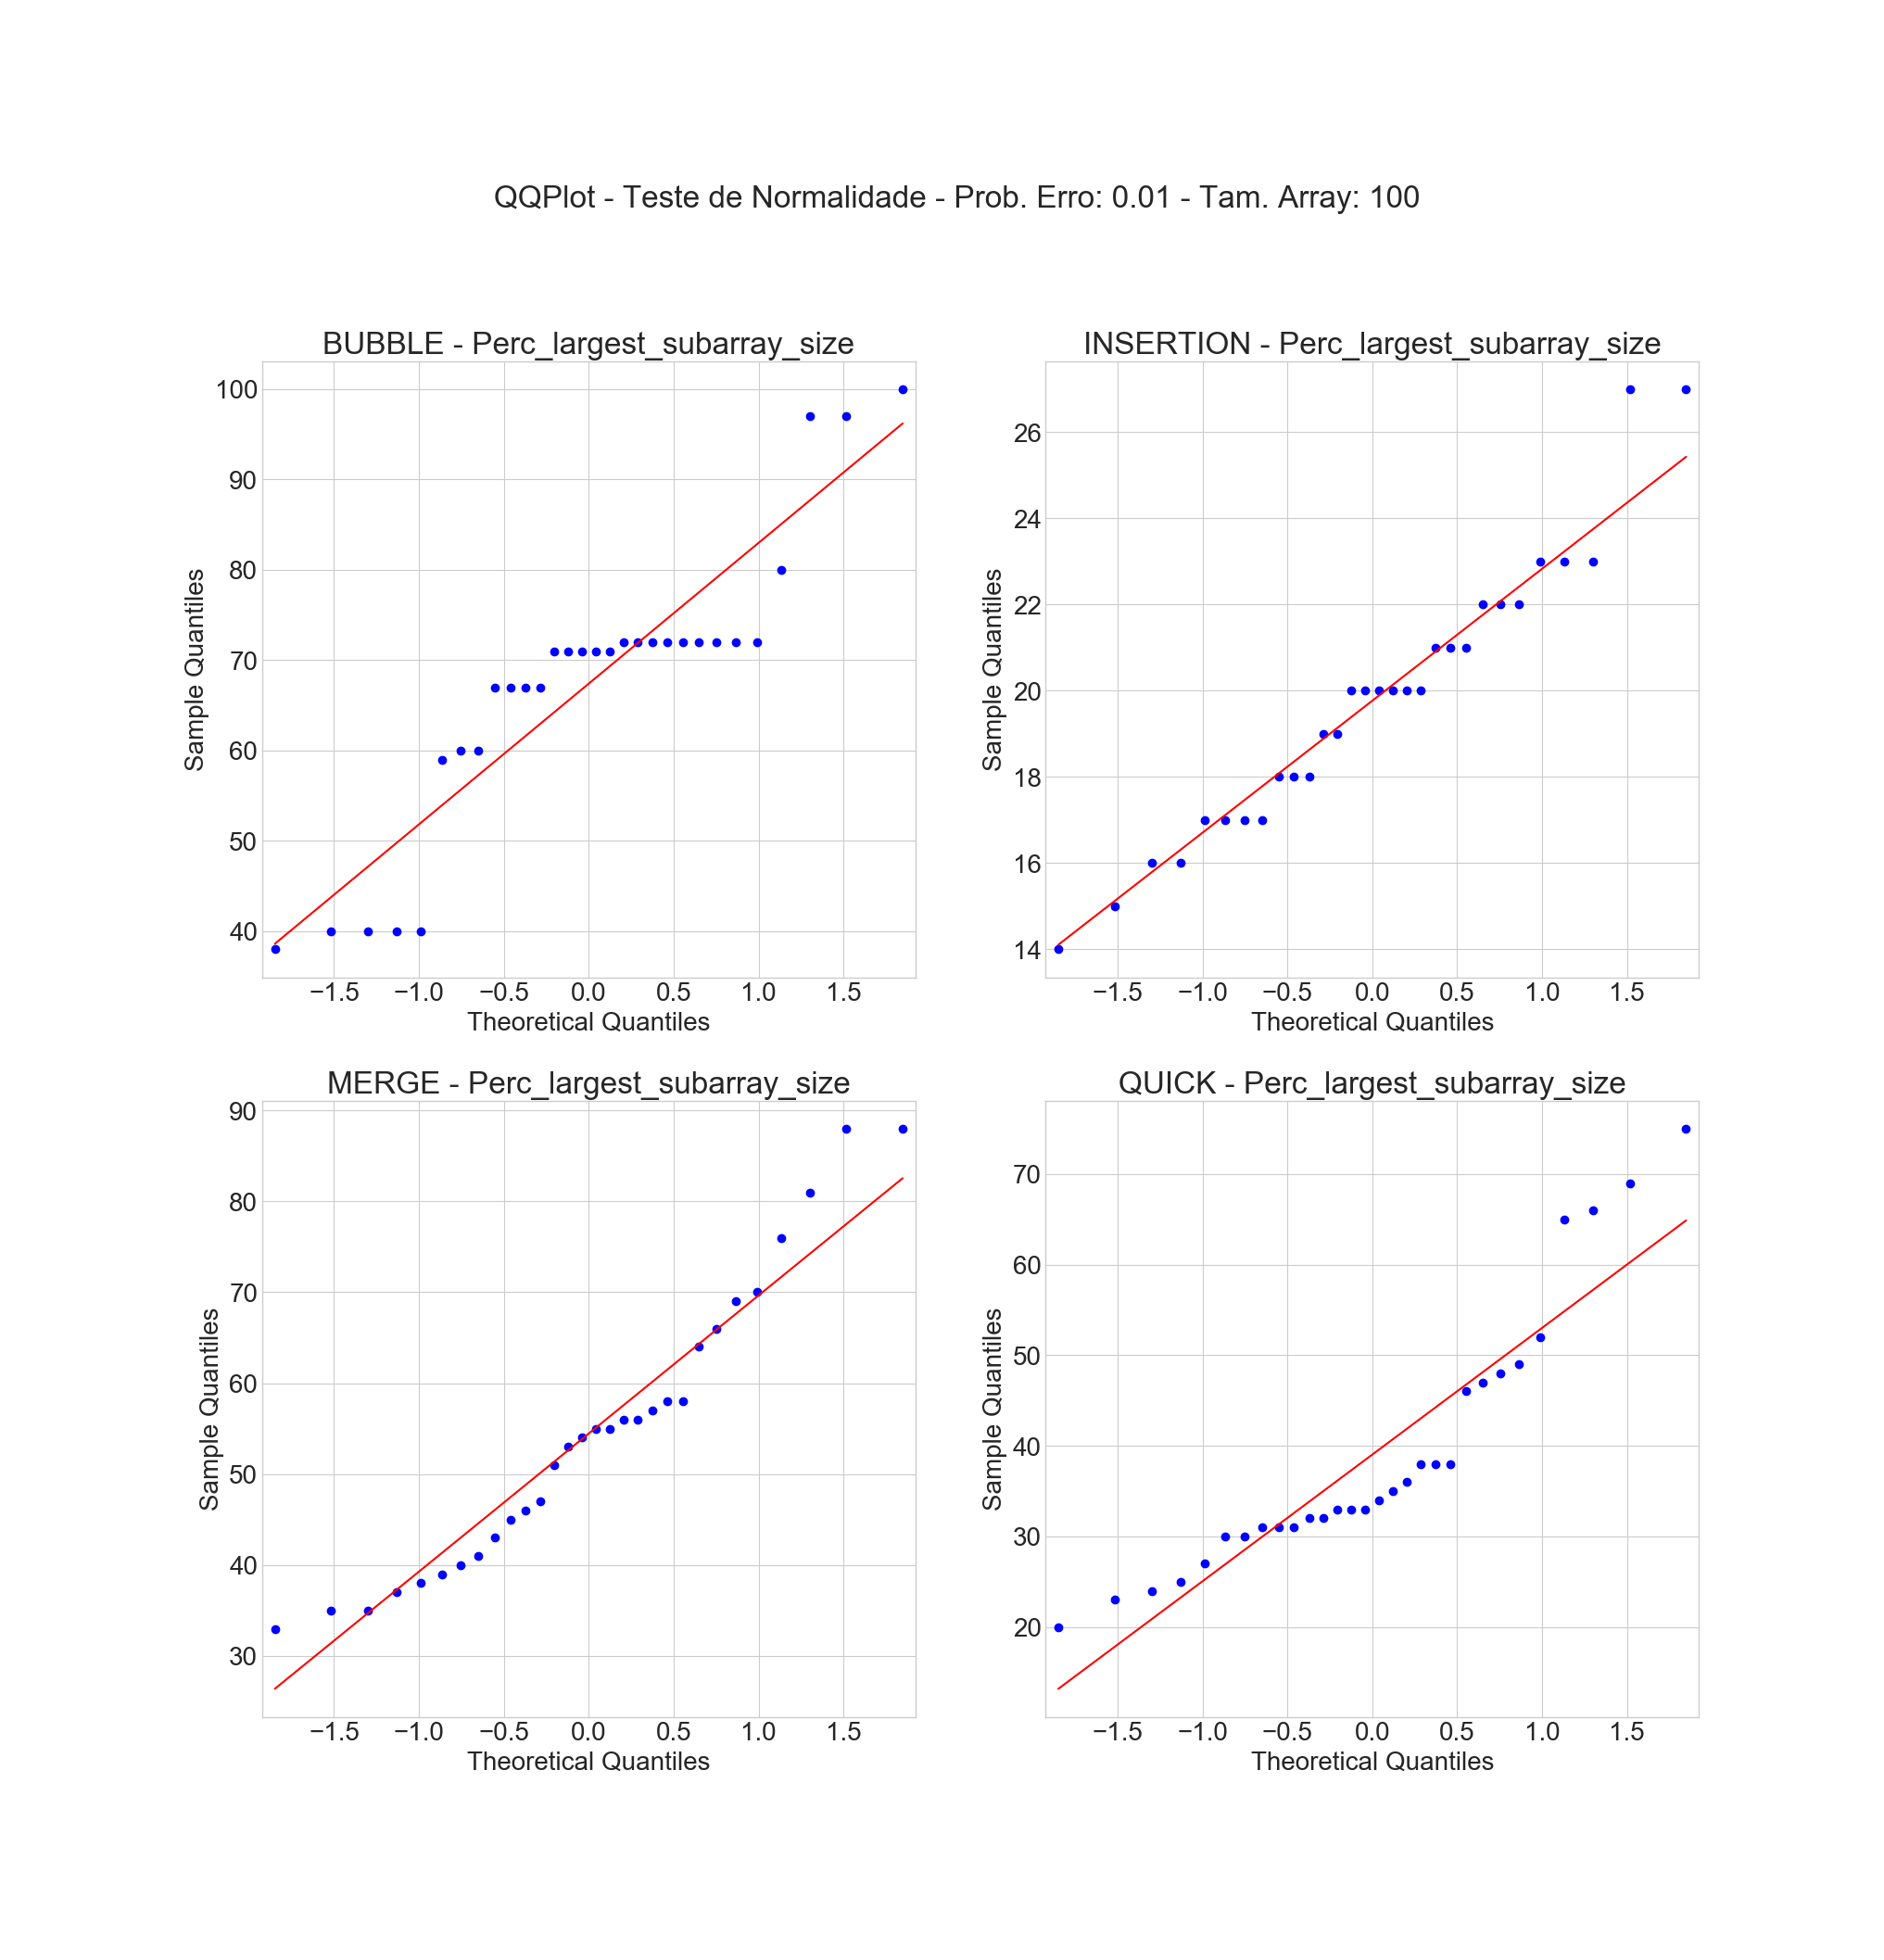
\includegraphics[scale=0.30]{figures/anova_prob_0_01_tam_100_Perc_largest_subarray_size.png}}
    \textsf{\caption[Q-Q plot for \%LSS with \textit{probability of failure} of 1\% and \textit{array size} of 100.]{Q-Q plot for \%LSS with \textit{probability of failure} of 1\% and \textit{array size} of 100.\label{fig-qqplot-lss-001-100}}}
 \end{figure}

 Figure \ref{fig-qqplot-ueq-001-100} shows the same graph for the dependent variable \textit{percentage of unordered elements quantity} considering same values for independent variables.

\begin{figure}[H]
    \centering
    \frame{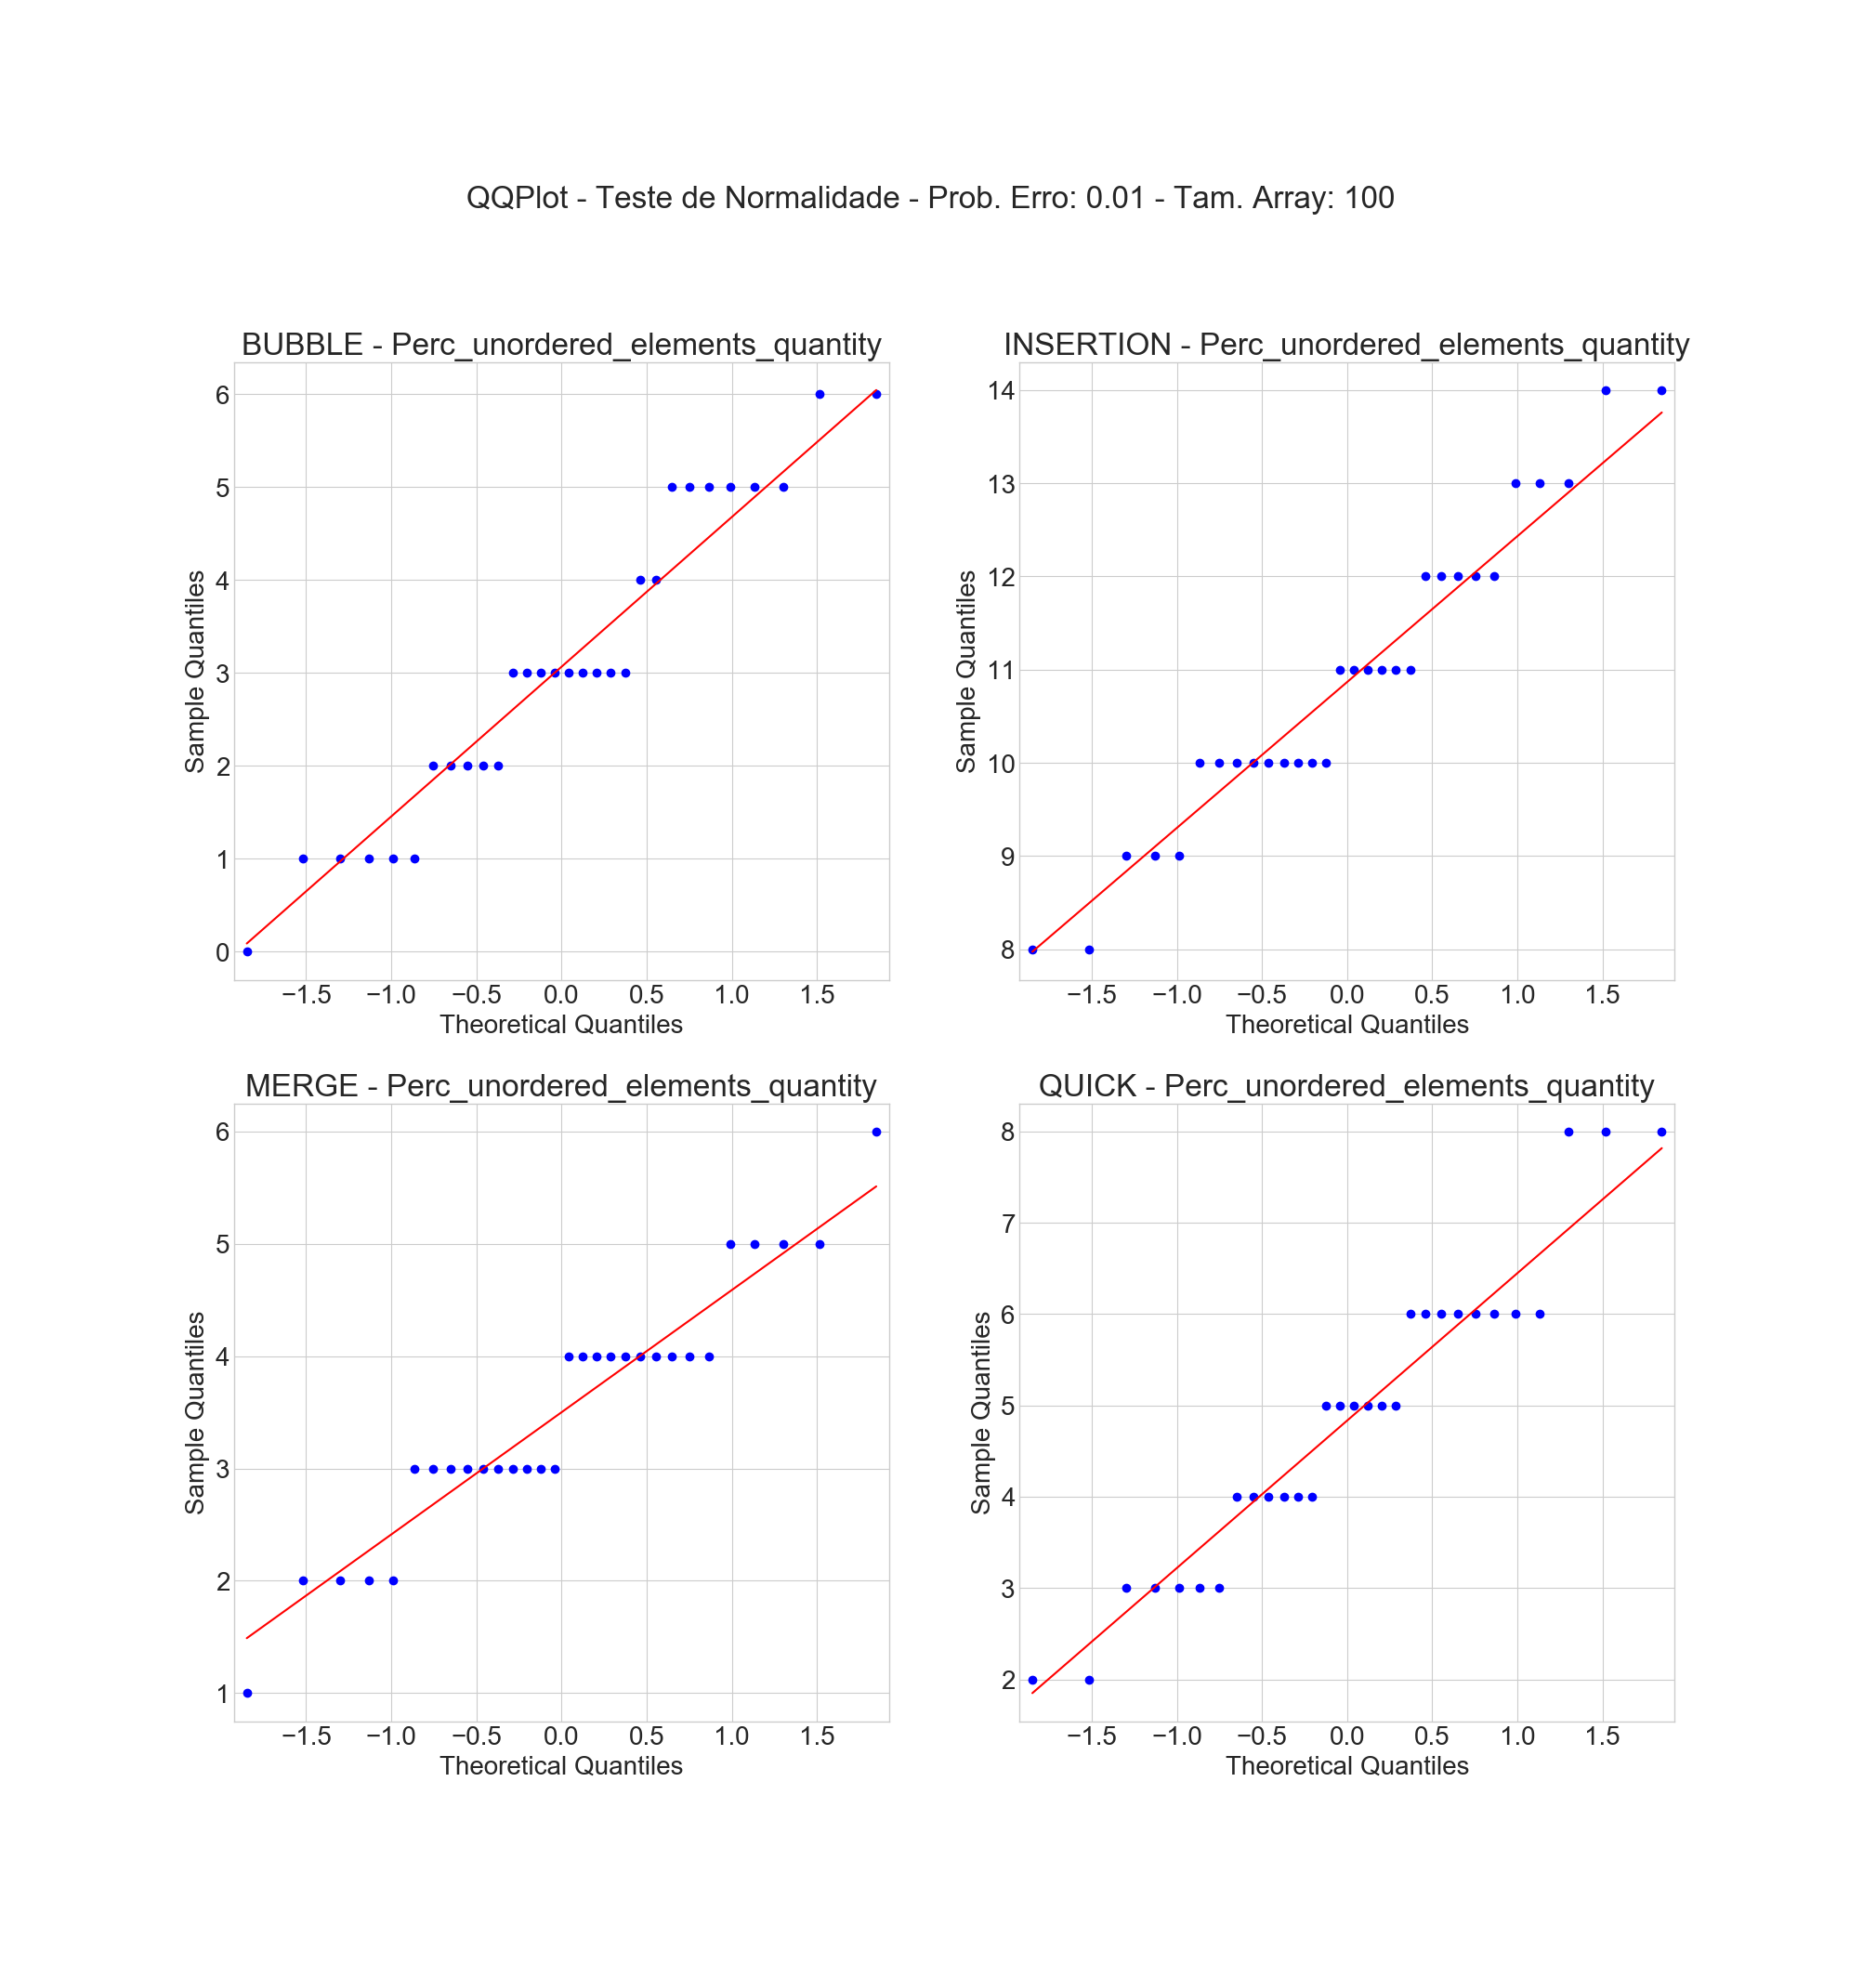
\includegraphics[scale=0.30]{figures/anova_prob_0_01_tam_100_Perc_unordered_elements_quantity.png}}
    \textsf{\caption[Q-Q plot for \%UEQ with \textit{probability of failure} of 1\% and \textit{array size} of 100.]{Q-Q plot for \%UEQ with \textit{probability of failure} of 1\% and \textit{array size} of 100.\label{fig-qqplot-ueq-001-100}}}
\end{figure}

Tables \ref{table-shapiro-test-lss-005-1000} and \ref{table-shapiro-test-ueq-005-1000} shows another examples of results we got running Shapiro-Wilk test. The independent variables assume these values: \textit{probability of failure} of 0.05 and \textit{array size} of 1000. The bold \textit{p-values} confirms that the data is normally distributed.

\begin{table}[H]
    \parbox{.45\linewidth}{
        \caption{Shapiro-Wilk test for \%LSS with \textit{probability of failure} of 5\% and \textit{array size} of 1000.}
        \begin{center}
        \begin{tabular}{|c|c|c|}
        \hline
        \textbf{Algorithm} & \textbf{W} & \textbf{p-value} \\
        \hline
        Bubblesort & 0.891642 & 0.0052 \\
        \hline
        Insertion Sort & 0.921918 & 0.0300 \\
        \hline
        Mergesort & 0.878308 & 0.0025 \\
        \hline
        Quicksort & 0.917583 & 0.0232 \\
        \hline
        \end{tabular}
        \label{table-shapiro-test-lss-005-1000}
        \end{center}
    }
    \hfill
    \parbox{.45\linewidth}{
        \caption{Shapiro-Wilk test for \%UEQ with \textit{probability of failure} of 5\% and \textit{array size} of 1000.}
        \begin{center}
        \begin{tabular}{|c|c|c|}
        \hline
        \textbf{Algorithm} & \textbf{W} & \textbf{p-value} \\
        \hline
        Bubblesort & 0.936459 & \textbf{0.0730} \\
        \hline
        Insertion Sort & 0.931681 & \textbf{0.0544} \\
        \hline
        Mergesort & 0.961920 & \textbf{0.3465} \\
        \hline
        Quicksort & 0.963954 & \textbf{0.3892} \\
        \hline
        \end{tabular}
        \label{table-shapiro-test-ueq-005-1000}
        \end{center}
    }
\end{table}

Other examples of distribution normality can be seen in Q-Q plot in Figures \ref{fig-qqplot-lss-005-1000} and Y below. The considered dependent variable is \textit{percentage of the largest subarray size} with a \textit{probability of failure} value of 5\% and \textit{array size} value of 10000 for all sorting algorithms.

\begin{figure}[H]
    \centering
    \frame{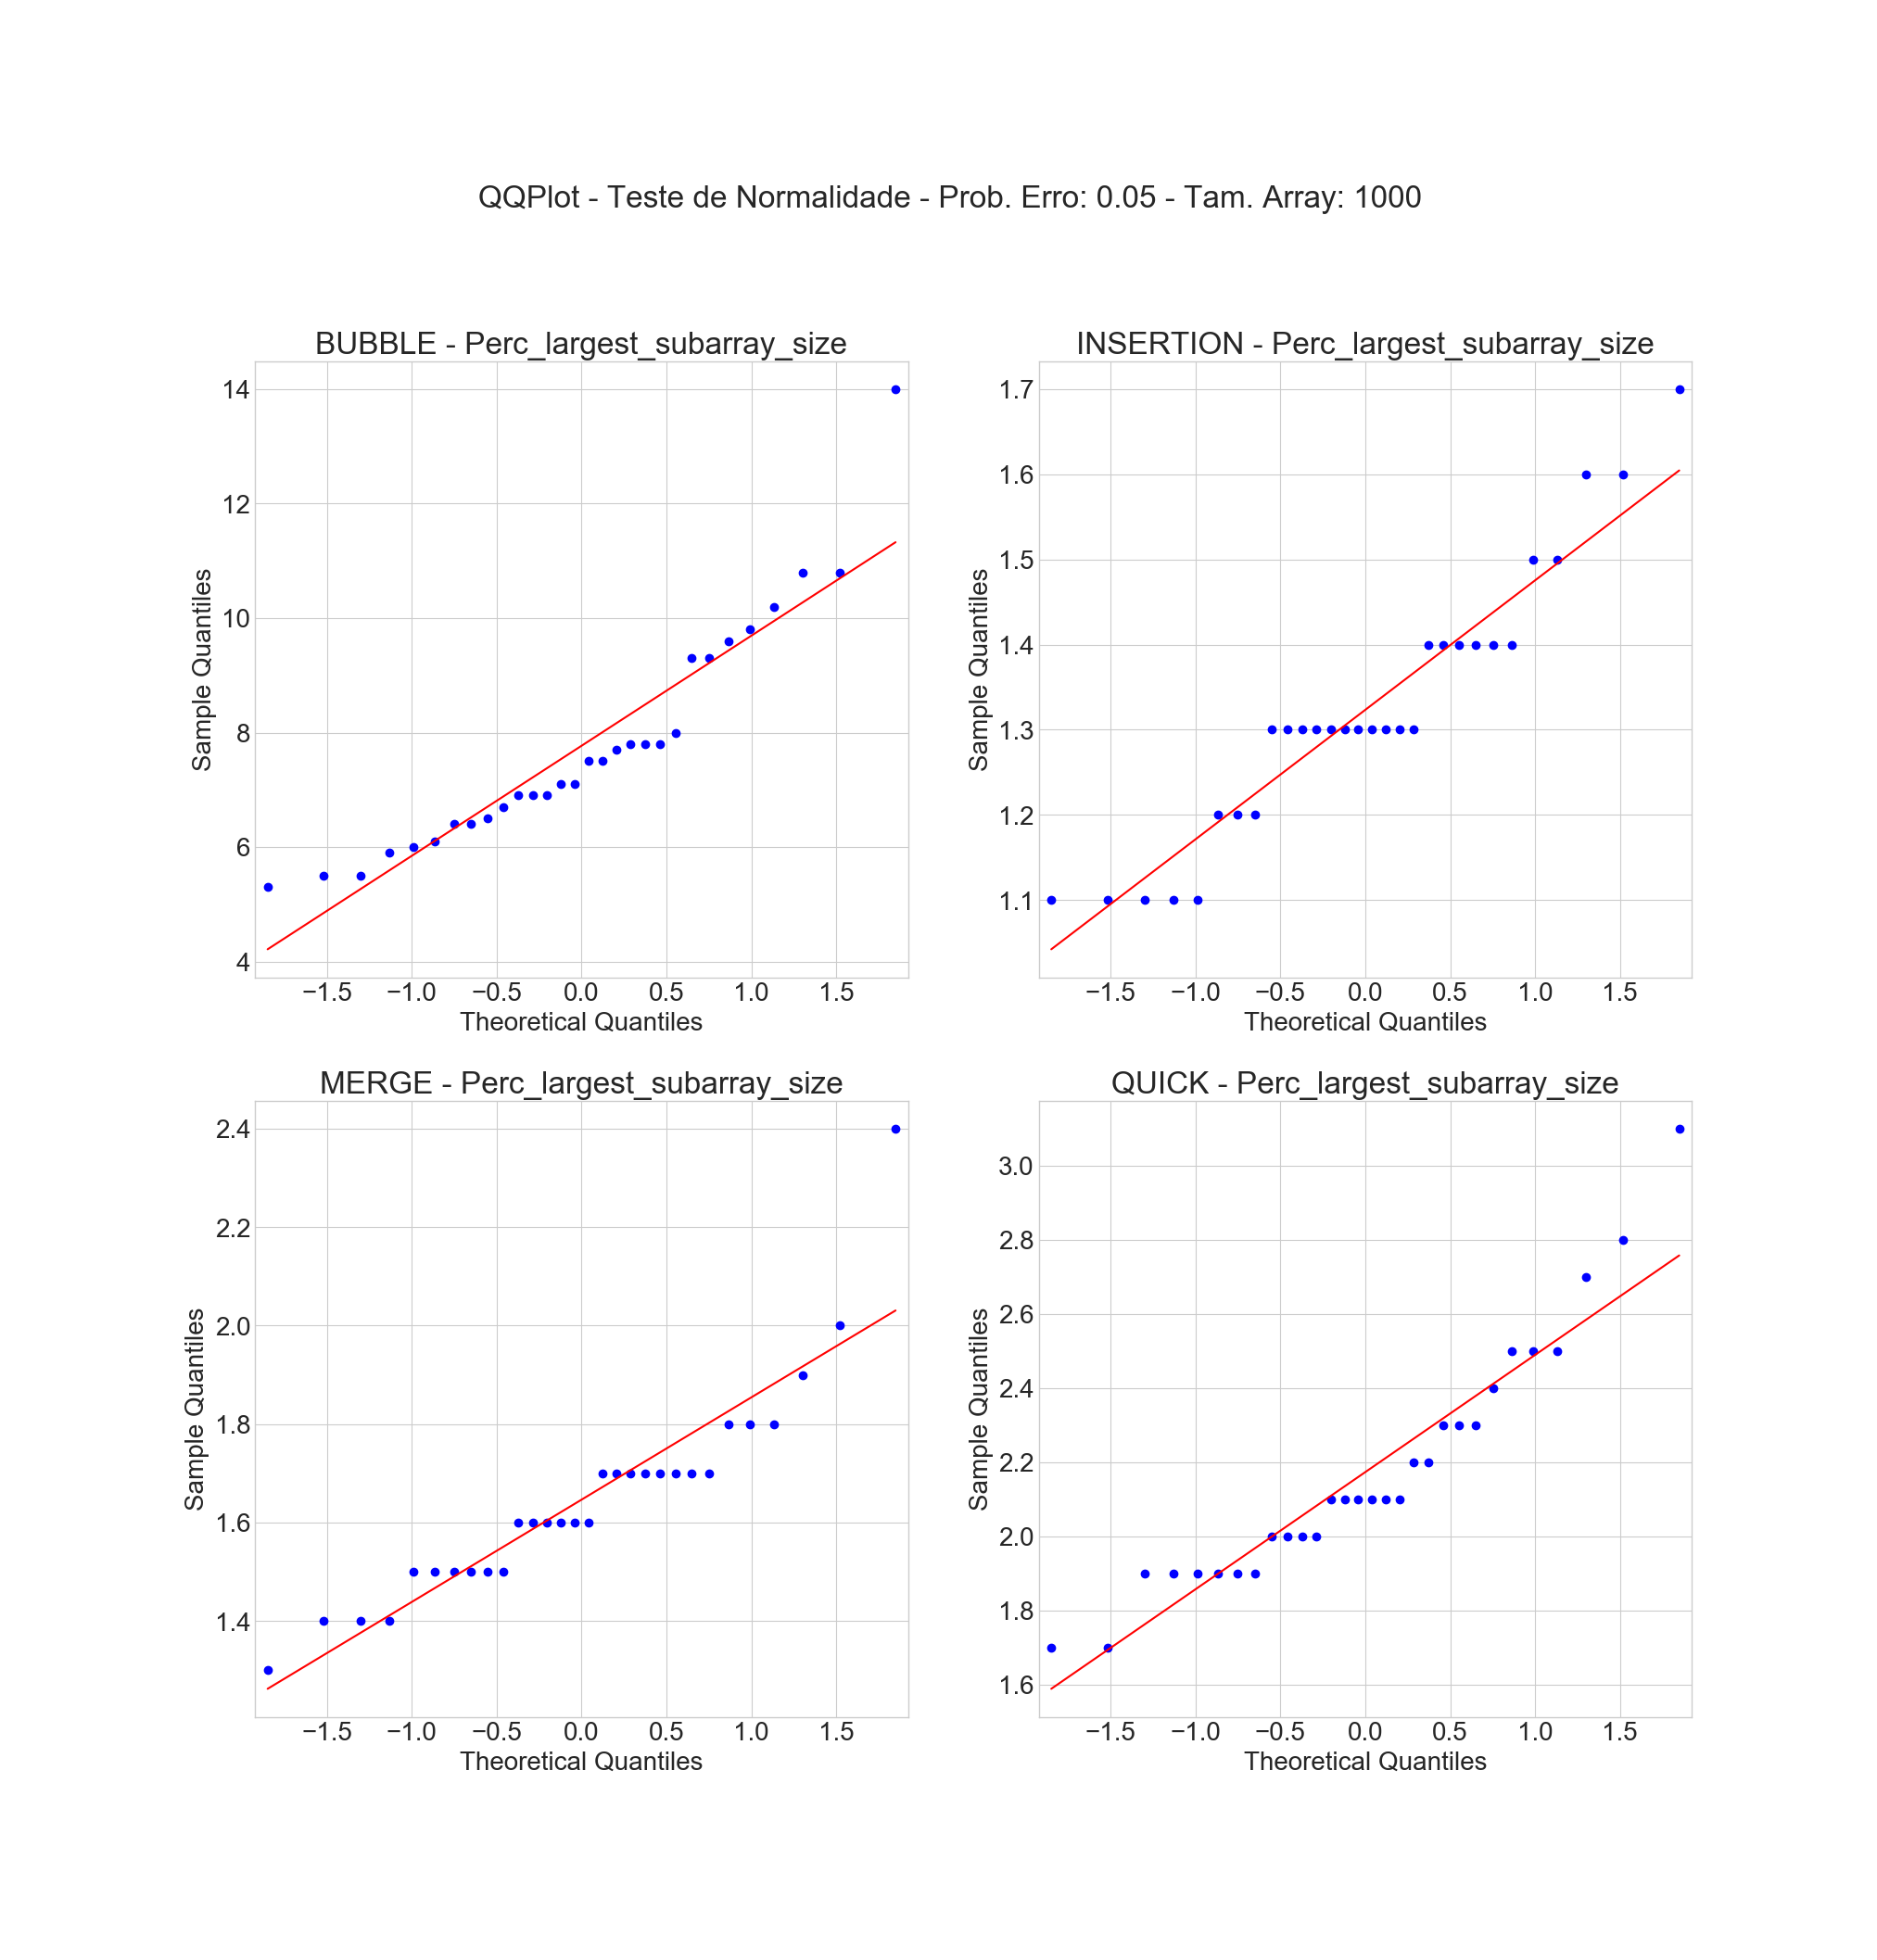
\includegraphics[scale=0.30]{figures/anova_prob_0_05_tam_1000_Perc_largest_subarray_size.png}}
    \textsf{\caption[Q-Q plot for \%LSS with \textit{probability of failure} of 5\% and \textit{array size} of 1000.]{Q-Q plot for \%LSS with \textit{probability of failure} of 5\% and \textit{array size} of 1000.\label{fig-qqplot-lss-005-1000}}}
 \end{figure}

 \begin{figure}[H]
    \centering
    \frame{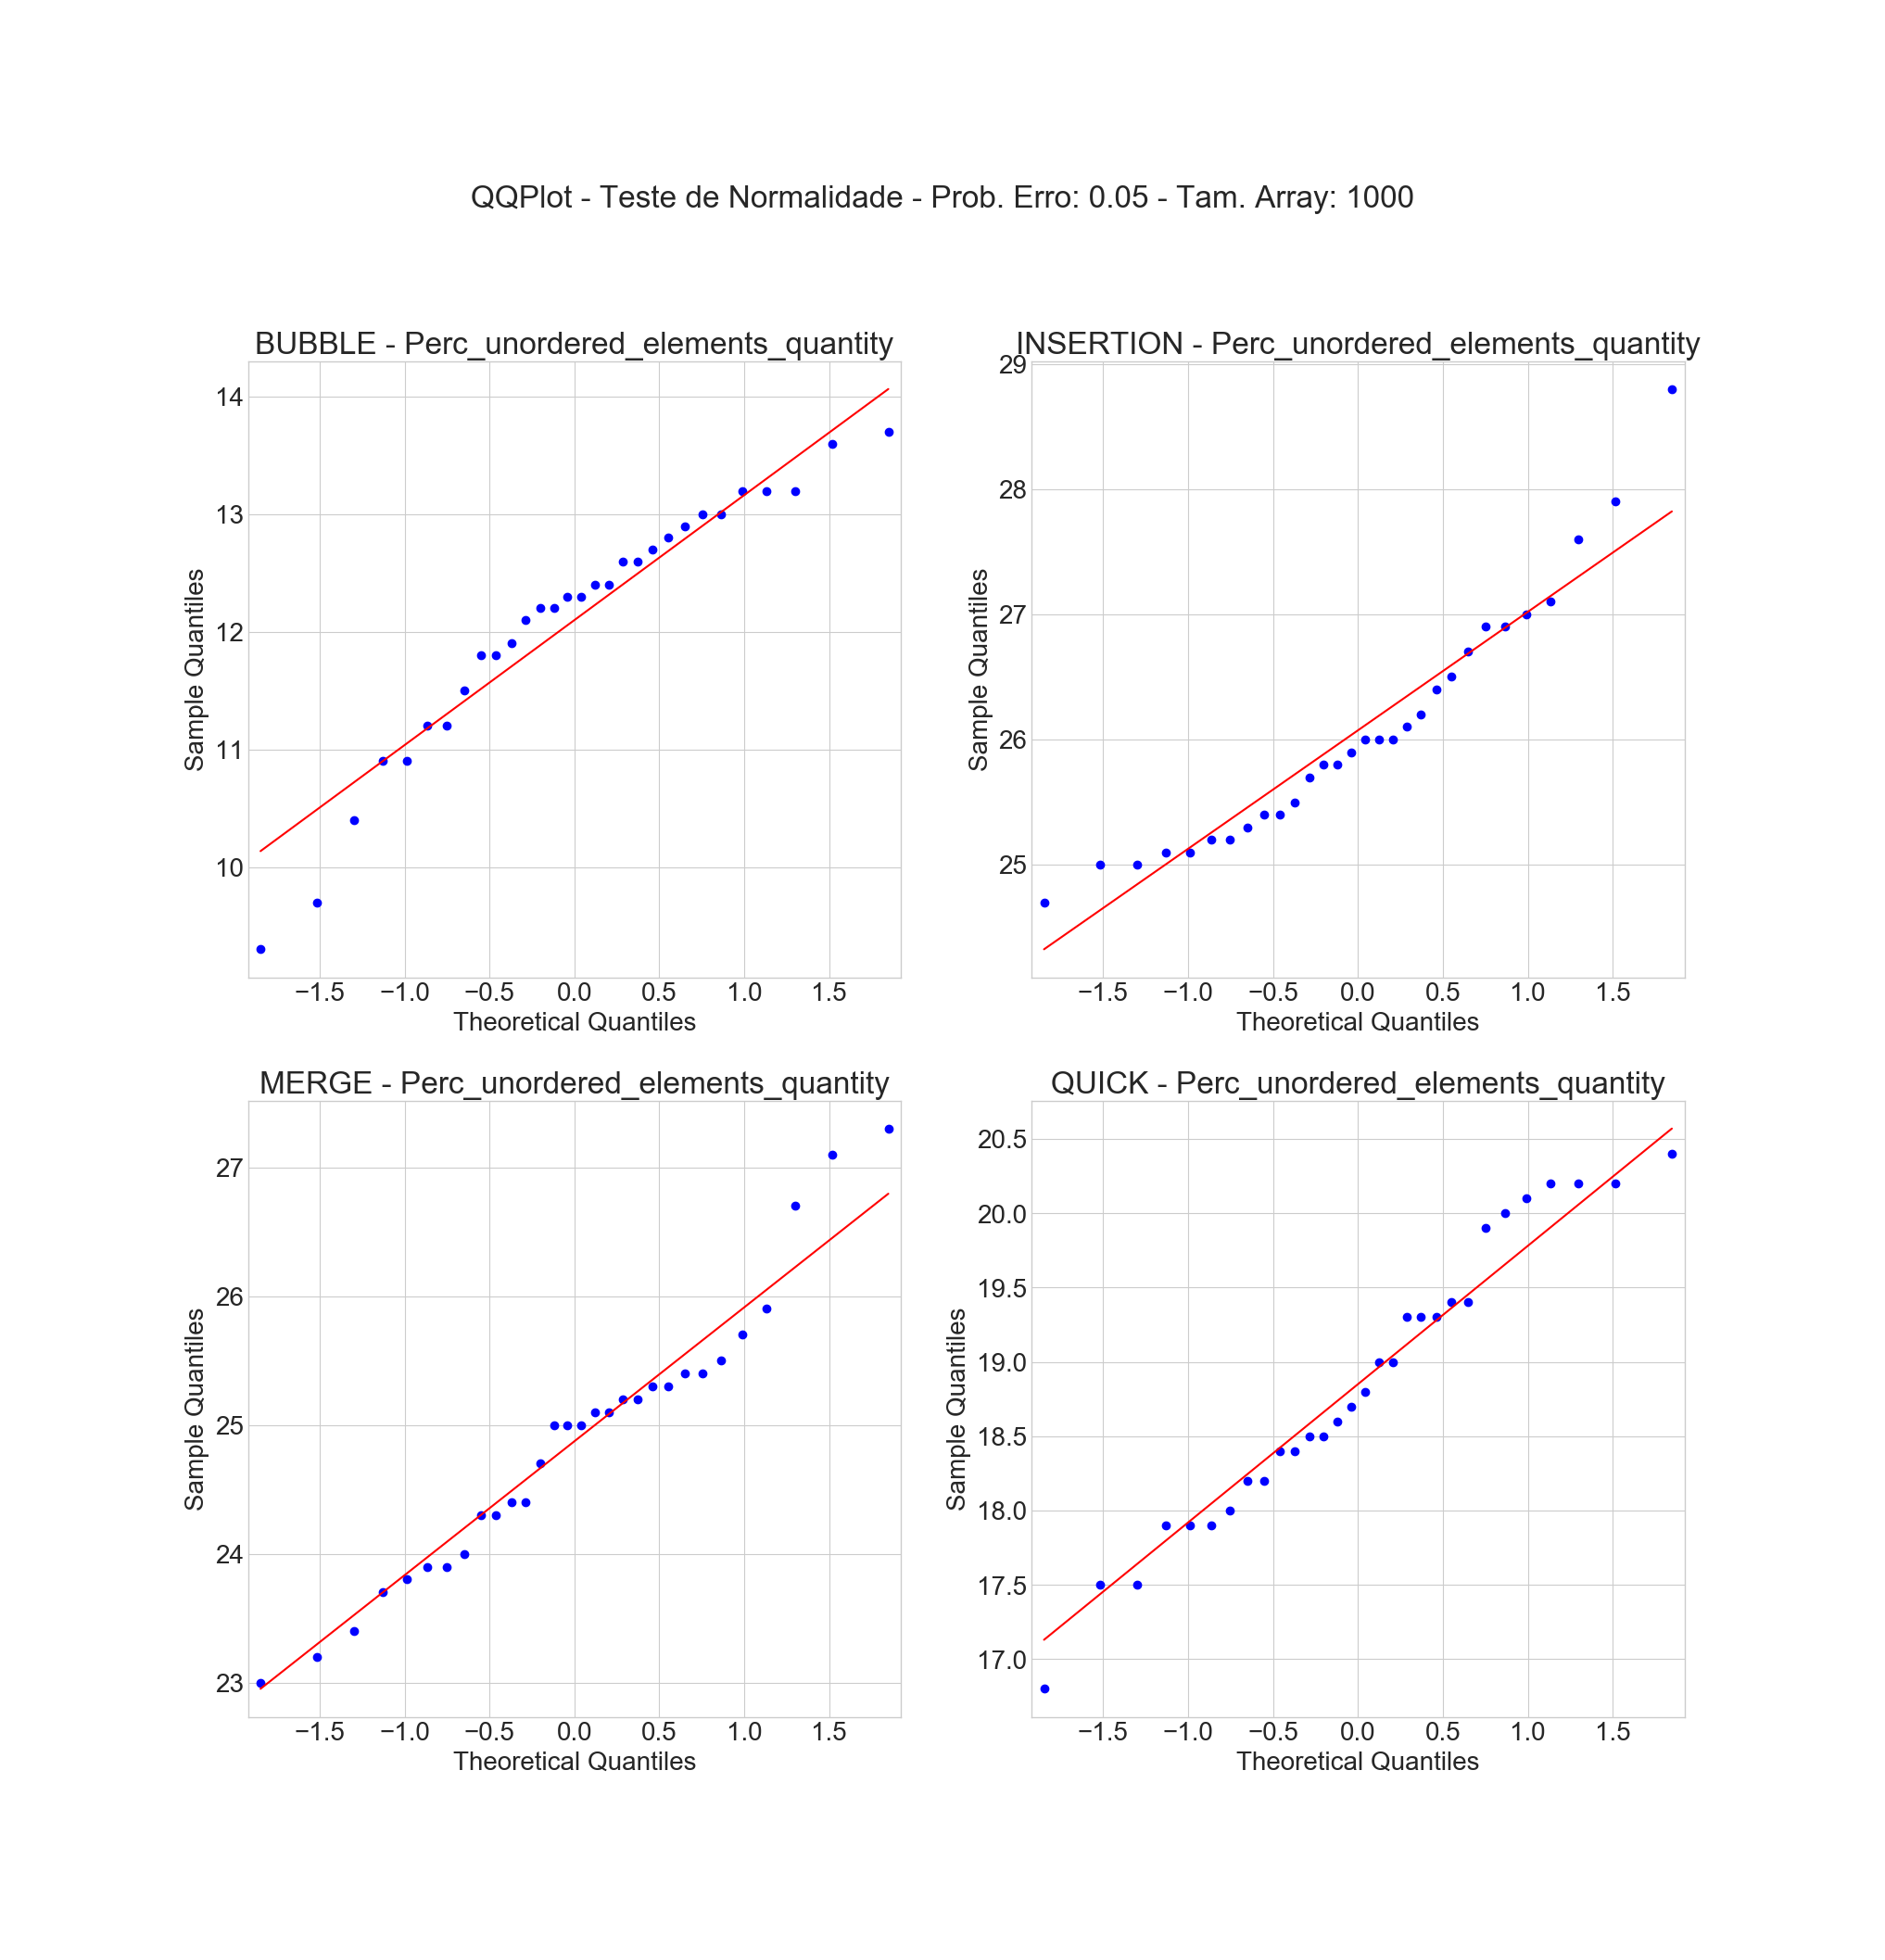
\includegraphics[scale=0.30]{figures/anova_prob_0_05_tam_1000_Perc_unordered_elements_quantity.png}}
    \textsf{\caption[Q-Q plot for \%UEQ with \textit{probability of failure} of 5\% and \textit{array size} of 1000.]{Q-Q plot for \%UEQ with \textit{probability of failure} of 5\% and \textit{array size} of 1000.\label{fig-qqplot-ueq-005-1000}}}
 \end{figure}

 \subsection{Hypothesis Testing}

 For hypothesis testing, we define a confidence degree of 95\%. As mentioned before, we only tested the hypothesis related to the dependent variable \%UEQ \textit{percentage of unordered elements quantity}. The hypothesis was:
 \begin{itemize}
     \item \textbf{Hypothesis 1}: For a given probability of failure and array size, tested algorithms will produce a different percentage of unordered elements quantity;
     \item \textbf{Hypothesis 3}: For each algorithm, the array size and probability of failure have a significative impact on the percentage of unordered elements quantity.
 \end{itemize}

 Because our dataset has 3 independent variables, we perform ANOVA method to simplify the hypothesis testing. This method allows comparing various groups of variables at the same time.

 \subsubsection{Testing Hypothesis 1}

We formulated the following hypothesis for the combination of independent variables \textit{probability of failure} and \textit{array size}:

\setcounter{hyp}{-1}
\begin{hyp} \label{hyp:a} There is no significant difference between algorithms related to variable \%UEQ.\end{hyp}
\begin{hyp} \label{hyp:b} There is significant difference between algorithms related to variable \%UEQ.\end{hyp}

After we run the testing method, we got the following results (Table \ref{tab-hypothesis1-testing}):

\begin{table}[H]
    \caption{Hypothesis 1 ANOVA results.}
    \begin{center}
    \begin{tabular}{|c|c|c|c|c|}
    \hline
    \multirow{2}{*}{\hfill}&\multicolumn{4}{|c|}{\textbf{Probablity of Failure = 1\% and Array Size = 100}} \\
    \cline{2-5}
    &\textbf{\textit{sum\_sq}} & \textbf{\textit{df}} & \textbf{\textit{F}} & \textbf{\textit{PR(>F)}} \\
    \hline
    algorithm & 1174.466667 & 3.0 & 171.368721 & \textbf{1.845762e-42} \\
    \hline
    residual & 265.000000 & 116.0 & & \\
    \hline
    \multirow{2}{*}{\hfill}&\multicolumn{4}{|c|}{\textbf{Probablity of Failure = 1\% and Array Size = 1000}} \\
    \cline{2-5}
    &\textbf{\textit{sum\_sq}} & \textbf{\textit{df}} & \textbf{\textit{F}} & \textbf{\textit{PR(>F)}} \\
    \hline
    algorithm & 1635.180250 & 3.0 & 1817.615579 & \textbf{2.610034e-97} \\
    \hline
    residual & 34.785667 & 116.0 & & \\
    \hline
    \multirow{2}{*}{\hfill}&\multicolumn{4}{|c|}{\textbf{Probablity of Failure = 1\% and Array Size = 10000}} \\
    \cline{2-5}
    &\textbf{\textit{sum\_sq}} & \textbf{\textit{df}} & \textbf{\textit{F}} & \textbf{\textit{PR(>F)}} \\
    \hline
    algorithm & 1948.204989 & 3.0 & 15831.708335 & \textbf{2.332995e-151} \\
    \hline
    residual & 4.758210 & 116.0 & & \\
    \hline
    \multirow{2}{*}{\hfill}&\multicolumn{4}{|c|}{\textbf{Probablity of Failure = 2\% and Array Size = 100}} \\
    \cline{2-5}
    &\textbf{\textit{sum\_sq}} & \textbf{\textit{df}} & \textbf{\textit{F}} & \textbf{\textit{PR(>F)}} \\
    \hline
    algorithm & 1106.5 & 3.0 & 88.617785 & \textbf{7.054900e-30} \\
    \hline
    residual & 482.8 & 116.0 & & \\
    \hline
    \multirow{2}{*}{\hfill}&\multicolumn{4}{|c|}{\textbf{Probablity of Failure = 2\% and Array Size = 1000}} \\
    \cline{2-5}
    &\textbf{\textit{sum\_sq}} & \textbf{\textit{df}} & \textbf{\textit{F}} & \textbf{\textit{PR(>F)}} \\
    \hline
    algorithm & 2286.83025 & 3.0 & 1990.144336 & \textbf{1.507899e-99} \\
    \hline
    residual & 44.43100 & 116.0 & & \\
    \hline
    \multirow{2}{*}{\hfill}&\multicolumn{4}{|c|}{\textbf{Probablity of Failure = 2\% and Array Size = 10000}} \\
    \cline{2-5}
    &\textbf{\textit{sum\_sq}} & \textbf{\textit{df}} & \textbf{\textit{F}} & \textbf{\textit{PR(>F)}} \\
    \hline
    algorithm & 3081.306943 & 3.0 & 18442.105239 & \textbf{3.406264e-155} \\
    \hline
    residual & 6.460427 & 116.0 & & \\
    \hline
    \multirow{2}{*}{\hfill}&\multicolumn{4}{|c|}{\textbf{Probablity of Failure = 5\% and Array Size = 100}} \\
    \cline{2-5}
    &\textbf{\textit{sum\_sq}} & \textbf{\textit{df}} & \textbf{\textit{F}} & \textbf{\textit{PR(>F)}} \\
    \hline
    algorithm & 2274.291667 & 3.0 & 225.58173 & \textbf{3.104916e-48} \\
    \hline
    residual & 389.833333 & 116.0 & & \\
    \hline
    \multirow{2}{*}{\hfill}&\multicolumn{4}{|c|}{\textbf{Probablity of Failure = 5\% and Array Size = 1000}} \\
    \cline{2-5}
    &\textbf{\textit{sum\_sq}} & \textbf{\textit{df}} & \textbf{\textit{F}} & \textbf{\textit{PR(>F)}} \\
    \hline
    algorithm & 3704.037583 & 3.0 & 1202.21591 & \textbf{3.625400e-87} \\
    \hline
    residual & 119.132333 & 116.0 & & \\
    \hline
    \multirow{2}{*}{\hfill}&\multicolumn{4}{|c|}{\textbf{Probablity of Failure = 5\% and Array Size = 10000}} \\
    \cline{2-5}
    &\textbf{\textit{sum\_sq}} & \textbf{\textit{df}} & \textbf{\textit{F}} & \textbf{\textit{PR(>F)}} \\
    \hline
    algorithm & 4948.821397 & 3.0 & 19487.120298 & \textbf{1.402080e-156} \\
    \hline
    residual & 9.819533 & 116.0 & & \\
    \hline
    \end{tabular}
    \label{tab-hypothesis1-testing}
    \end{center}
\end{table}

Based on these results, we reject the null hypothesis ($H_{0}$) for all testing combinations. Therefore, we can affirm with 95\% of confidence that there is a significant difference between algorithms related do variable \%UEQ.

\subsubsection{Testing Hypothesis 3}

We formulated the following hypothesis for all algorithms considered in this work:

\setcounter{hyp}{-1}
\begin{hyp} \label{hyp:a} The values of variables \textit{probability of failure} and \textit{array size} don't have a significant impact on values of \%UEQ variable.\end{hyp}
\begin{hyp} \label{hyp:b} The values of variables \textit{probability of failure} and \textit{array size} have a significant impact on values of \%UEQ variable.\end{hyp}

After we run the testing method, we got the following results (Table \ref{tab-hypothesis3-testing}):

\begin{table}[H]
    \caption{Hypothesis 3 ANOVA results}
    \begin{center}
    \begin{tabular}{|c|c|c|c|c|}
    \hline
    \multirow{2}{*}{\hfill}&\multicolumn{4}{|c|}{\textbf{Bubblesort}} \\
    \cline{2-5}
    &\textbf{\textit{sum\_sq}} & \textbf{\textit{df}} & \textbf{\textit{F}} & \textbf{\textit{PR(>F)}} \\
    \hline
    size\_of\_array & 0.019548 & 1.0 & 0.01350 & \textbf{0.90759} \\
    \hline
    probability\_of\_failure & 3590.644437 & 1.0 & 2479.71637 & \textbf{7.570027e-137} \\
    \hline
    residual & 385.169623 & 266.0 & &  \\
    \hline
    \multirow{2}{*}{\hfill}&\multicolumn{4}{|c|}{\textbf{Mergesort}} \\
    \cline{2-5}
    &\textbf{\textit{sum\_sq}} & \textbf{\textit{df}} & \textbf{\textit{F}} & \textbf{\textit{PR(>F)}} \\
    \hline
    size\_of\_array & 1784.873256 & 1.0 & 383.585800 & \textbf{1.702008e-53} \\
    \hline
    probability\_of\_failure & 13009.963175 & 1.0 & 2795.961630 & \textbf{3.801570e-143} \\
    \hline
    residual & 1237.731651 & 266.0 & &  \\
    \hline
    \multirow{2}{*}{\hfill}&\multicolumn{4}{|c|}{\textbf{Quicksort}} \\
    \cline{2-5}
    &\textbf{\textit{sum\_sq}} & \textbf{\textit{df}} & \textbf{\textit{F}} & \textbf{\textit{PR(>F)}} \\
    \hline
    size\_of\_array & 121.551362 & 1.0 & 32.964196 & \textbf{2.556033e-08} \\
    \hline
    probability\_of\_failure & 5626.955128 & 1.0 & 1526.005558 & \textbf{3.457996e-112} \\
    \hline
    residual & 980.841817 & 266.0 & &  \\
    \hline
    \multirow{2}{*}{\hfill}&\multicolumn{4}{|c|}{\textbf{Insertionsort}} \\
    \cline{2-5}
    &\textbf{\textit{sum\_sq}} & \textbf{\textit{df}} & \textbf{\textit{F}} & \textbf{\textit{PR(>F)}} \\
    \hline
    size\_of\_array & 309.843991 & 1.0 & 75.905868 & \textbf{3.236586e-16} \\
    \hline
    probability\_of\_failure & 6806.075083 & 1.0 & 1667.358570 & \textbf{1.414758e-116} \\
    \hline
    residual & 1085.798822 & 116.0 & & \\
    \hline
    \end{tabular}
    \label{tab-hypothesis3-testing}
    \end{center}
\end{table}

Based on these results, we reject the null hypothesis ($H_{0}$) for algorithms Mergesort, Quicksort, and Insertion sort. Therefore, we can affirm with 95\% of confidence that the values of variables \textit{probability of failure} and \textit{array size} have a significant impact on values of \%UEQ variable.

For Bubblesort algorithm, however, there is no confidence to reject the null hypothesis ($H_{0}$). Analyzing the result, we can affirm with 95\% of confidence that the value of \textit{probability of failure} variable had a significant impact on the value of the dependent variable \%UEQ. But we can not affirm the same related to independent variable \textit{array size}. These results demonstrate that, for the Bubblesort algorithm, the array sizes used in this experiment were not decisive to define values concerning the percentage of unordered elements quantity.

\subsection{Performance analysis related to \textit{percentage of unordered elements quantity} variable}

In this section, we present an analysis of overall performance related to dependent variable \textit{percentage of unordered elements quantity}. To help this analysis, we show below 3 bar graphs, each of these for a different value of \textit{probability of failure} independent variable. These graphs show information about values of \%UEQ variable grouped by \textit{array size} and \textit{sorting algorithm} variables. Figures \ref{fig-barplot-pof-001}, \ref{fig-barplot-pof-002}, and \ref{fig-barplot-pof-005} below exhibit these graphs.

The bars in each graph represent the sample mean value for variable \%UEQ inside each group. Above each bar, there is a vertical line that indicates the lower and upper limits of a confidence interval for a significance level of 5\% ($\alpha = 0.05$).

\begin{figure}[H]
    \centering
    \frame{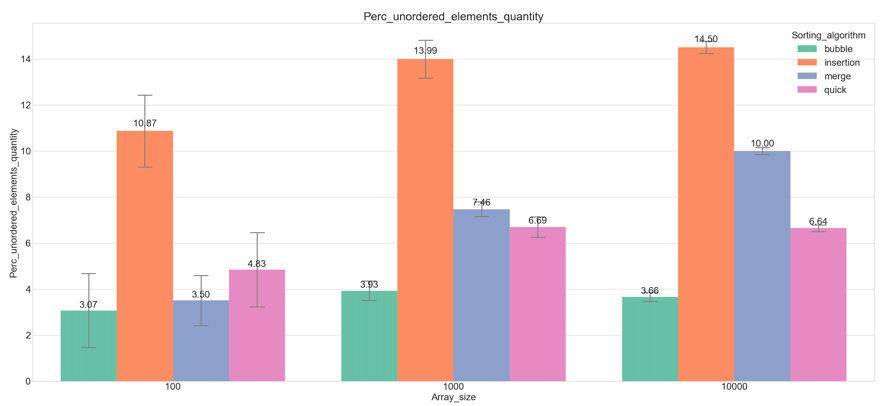
\includegraphics[scale=1.15]{figures/Barplot_Estatisticas_por_Algoritmo_Prob_0_01.png}}
    \textsf{\caption[Data for \textit{probability of failure} of 1\%.]{Data for \textit{probability of failure} of 1\%.\label{fig-barplot-pof-001}}}
 \end{figure}

 \begin{figure}[H]
    \centering
    \frame{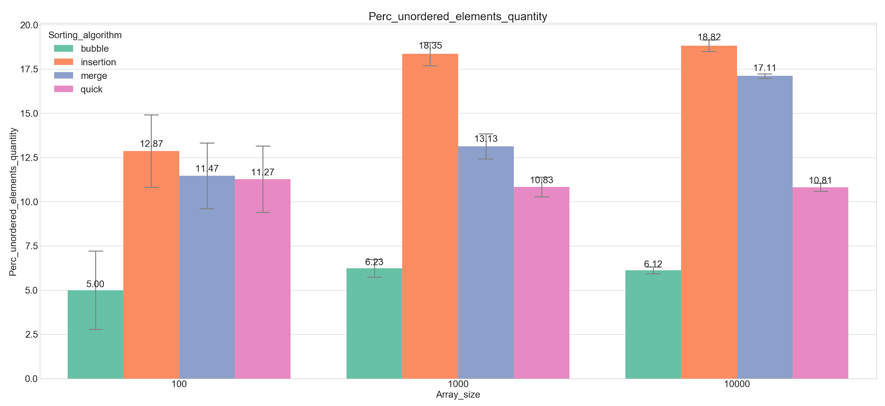
\includegraphics[scale=1.15]{figures/Barplot_Estatisticas_por_Algoritmo_Prob_0_02.png}}
    \textsf{\caption[Data for \textit{probability of failure} of 2\%.]{Data for \textit{probability of failure} of 2\%.\label{fig-barplot-pof-002}}}
 \end{figure}

 \begin{figure}[H]
    \centering
    \frame{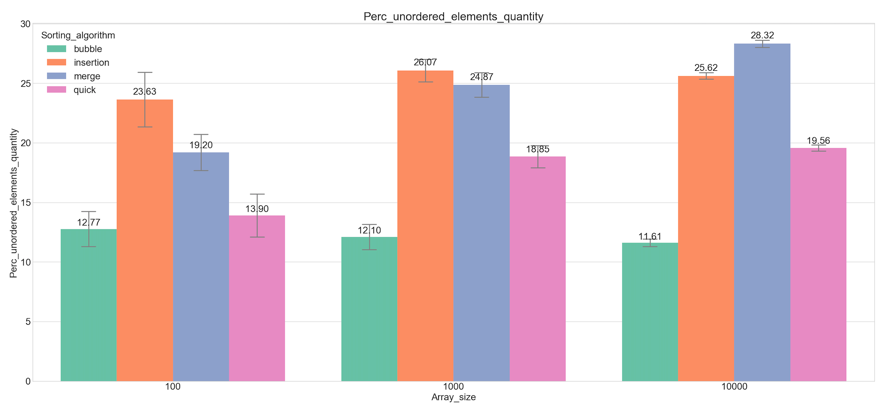
\includegraphics[scale=1.15]{figures/Barplot_Estatisticas_por_Algoritmo_Prob_0_05.png}}
    \textsf{\caption[Data for \textit{probability of failure} of 5\%.]{Data for \textit{probability of failure} of 5\%.\label{fig-barplot-pof-005}}}
\end{figure}

Considering the data in the graphs, we can conclude that Bubblesort generates lower mean value for variable \%UEQ for all defined combinations (\textit{probability of failure} X \textit{array size} X \textit{sorting algorithm}). These data demonstrate that Bubblesort was the less affected algorithm by the memory faults simulated in this experiment. We believe that this fact happened because of the operation of the algorithm itself, where all elements order are verified each iteration, causing an element incorrectly positioned in an iteration (because of a memory fault) can have its location corrected in an upcoming iteration.

Related to Bubblesort yet, we could identify that despite different sizes of input arrays (100, 1000, and 10000), there was not a significant impact on the mean value obtained for \%UEQ variable, proving what we verify with ANOVA when doing hypothesis 3 testing for this algorithm.

\section{Linear Regression}

The linear regression analysis consists of statistical analysis to verify the existence of a functional relationship between a dependent variable with one or more independent variables. In other words, this analysis consists of obtaining a linear equation that tries to explain the variation from the dependent variable by variation from the independent variable level.

The statistical model for this case should be:
\begin{equation} 
    \label{eqn_example}
    y = a.x + b
\end{equation}

Where $y$ represents the dependent variable, $a$ represents the line slope of the linear model, and $b$ represents the y-axis intercept. The regression line is a method to calculate the parameters $a$ and $b$.

The determination coefficient, frequently called $R^2$, or simply $r^2$, for the linear regression case, provide auxiliary information to the analysis of the result of regression variance, as a way to verify if the proposed model is suitable or not to describe the phenomenon.

In this work, we verified how close is the relationship between the \textit{probability of failure} independent variable and the other dependent variables: \%LSS and \%UEQ to a linear equation.

To discover an equation that represents the studied phenomenon, we could build a graph, called \textit{Scatter Plot}, to verify by visualization how is the variation between the dependent and independent variables.

To discover an equation that represents the studied phenomenon, we could build a graph, called scatter plot, to verify by visualization how is the variation between the dependent and independent variables. Figures \ref{fig-linear-regression-scatter-plots-lss} and \ref{fig-linear-regression-scatter-plots-ueq} are the scatter plots for \%LSS and \%UEQ for each algorithm, respectively. In these figures, we can see the line from the linear equation from the estimated model that used the minimum mean square error as criteria. The red dotted line represents the bounds for 95\% of the confidence interval.

\begin{figure}[H]
    \centering
     \begin{subfigure}{.5\textwidth}
     \centering
     \frame{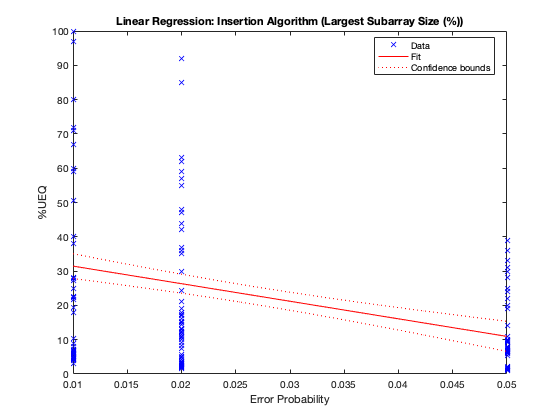
\includegraphics[scale=0.45]{figures/linear_regression_scatter_plot_lss_bubble.png}}
     \textsf{\caption[Bubblesort algorithm.]{Bubblesort algorithm.\label{fig-linear-regression-scatter-plot-lss-bubble}}}
     \end{subfigure}%
     \begin{subfigure}{.5\textwidth}
     \centering
     \frame{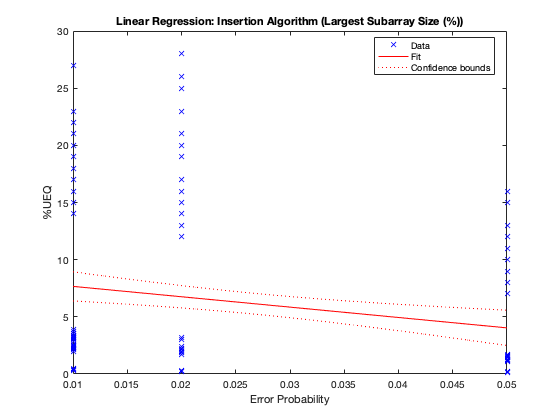
\includegraphics[scale=0.45]{figures/linear_regression_scatter_plot_lss_insertion.png}}
     \textsf{\caption[Insertionsort algorithm.]{Insertionsort algorithm.\label{fig-linear-regression-scatter-plot-lss-insertion}}}
     \end{subfigure}
     \begin{subfigure}{.5\textwidth}
     \centering
     \frame{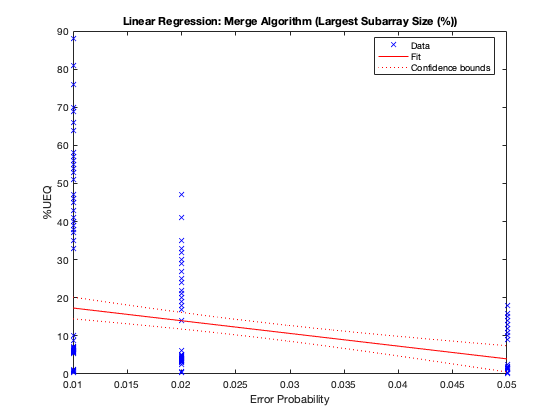
\includegraphics[scale=0.45]{figures/linear_regression_scatter_plot_lss_merge.png}}
     \textsf{\caption[Mergesort algorithm.]{Mergesort algorithm.\label{fig-linear-regression-scatter-plot-lss-merge}}}
     \end{subfigure}%
     \begin{subfigure}{.5\textwidth}
     \centering
     \frame{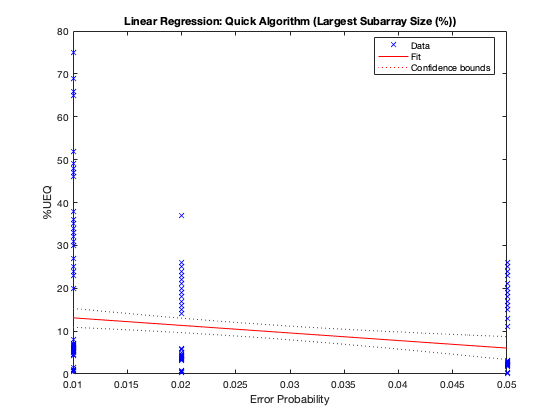
\includegraphics[scale=0.45]{figures/linear_regression_scatter_plot_lss_quick.png}}
     \textsf{\caption[Quicksort algorithm.]{Quicksort algorithm.\label{fig-linear-regression-scatter-plot-lss-quick}}}
     \end{subfigure}
     \caption{Scatter plot and the linear regression for \%LSS versus Probability of Failure.}
    \label{fig-linear-regression-scatter-plots-lss}
  \end{figure}

  \begin{figure}[H]
    \centering
     \begin{subfigure}{.5\textwidth}
     \centering
     \frame{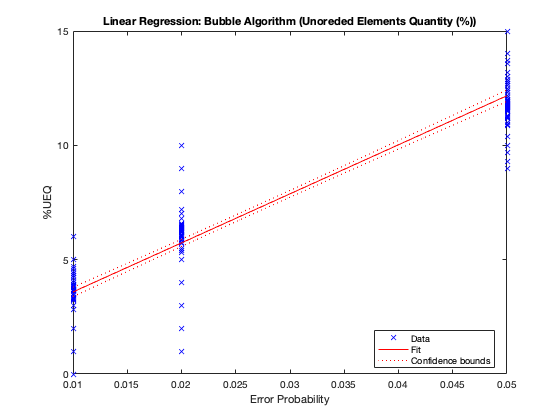
\includegraphics[scale=0.45]{figures/linear_regression_scatter_plot_ueq_bubble.png}}
     \textsf{\caption[Bubblesort algorithm.]{Bubblesort algorithm.\label{fig-linear-regression-scatter-plot-ueq-bubble}}}
     \end{subfigure}%
     \begin{subfigure}{.5\textwidth}
     \centering
     \frame{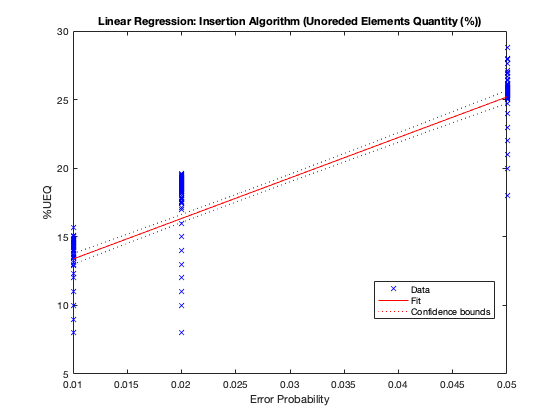
\includegraphics[scale=0.45]{figures/linear_regression_scatter_plot_ueq_insertion.png}}
     \textsf{\caption[Insertionsort algorithm.]{Insertionsort algorithm.\label{fig-linear-regression-scatter-plot-ueq-insertion}}}
     \end{subfigure}
     \begin{subfigure}{.5\textwidth}
     \centering
     \frame{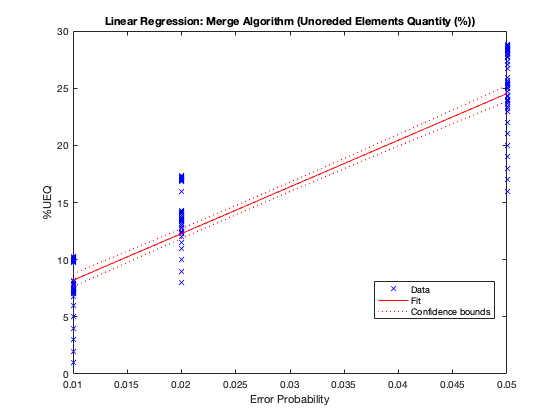
\includegraphics[scale=0.45]{figures/linear_regression_scatter_plot_ueq_merge.png}}
     \textsf{\caption[Mergesort algorithm.]{Mergesort algorithm.\label{fig-linear-regression-scatter-plot-ueq-merge}}}
     \end{subfigure}%
     \begin{subfigure}{.5\textwidth}
     \centering
     \frame{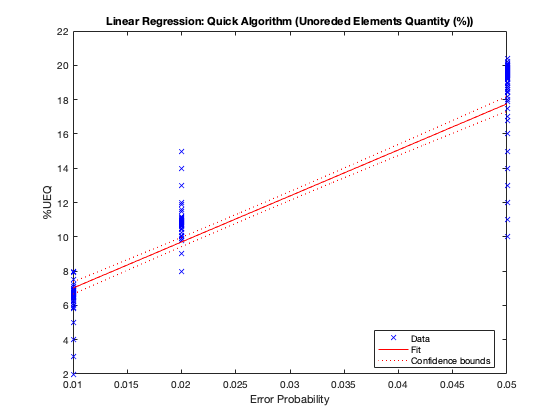
\includegraphics[scale=0.45]{figures/linear_regression_scatter_plot_ueq_quick.png}}
     \textsf{\caption[Quicksort algorithm.]{Quicksort algorithm.\label{fig-linear-regression-scatter-plot-ueq-quick}}}
     \end{subfigure}
     \caption{Scatter plot and the linear regression for \%UEQ versus Probability of Failure.}
    \label{fig-linear-regression-scatter-plots-ueq}
  \end{figure}

  However, we can verify that the points at scatter plots, don't have perfect adjust to the proposed math model line. There are, in major part, a great distance between the points at the plot and the model line. This distance happens because, in each probability of failure, we have many values of the dependent variable and with large dispersion. This situation explains why the determination coefficient $r^2$ has a low value in most of the cases.

  The Tables \ref{table-linear-regression-lss} and \ref{table-linear-regression-ueq} below shows the parameters for linear regression of both variables \%LSS and \%UEQ. For \%UEQ variable, we found better (from 0.809 to 0.899) $r^2$ than \%LSS (from 0.0499 to 0.141) variable for all algorithms.

  \begin{table}[H]
    \caption{Parameters from linear regression for the \%LSS variable.}
    \begin{center}
    \begin{tabular}{|c|c|c|c|c|}
    \hline
    \textbf{Parameter} & \textbf{Bubblesort} & \textbf{Quicksort} & \textbf{Mergesort} & \textbf{Insertionsort} \\
    \hline
    Intercept (b) & 36.576 & 14.86 & 20.651 & 8.5707 \\
    \hline
    Slope (a) & -512.32 & -176.4 & -333.64 & -90.711 \\
    \hline
    $r^2$ & 0.141 & 0.0499 & 0.101 & 0.0399 \\
    \hline
    Root Mean Squared Error (RMSE) & 21.5 & 13.1 & 17 & 7.59 \\
    \hline
    \end{tabular}
    \label{table-linear-regression-lss}
    \end{center}
\end{table}

\begin{table}[H]
    \caption{Parameters from linear regression for the \%UEQ variable.}
    \begin{center}
    \begin{tabular}{|c|c|c|c|c|}
    \hline
    \textbf{Parameter} & \textbf{Bubblesort} & \textbf{Quicksort} & \textbf{Mergesort} & \textbf{Insertionsort} \\
    \hline
    Intercept (b) & 1.4429 & 4.3258 & 4.1165 & 10.426 \\
    \hline
    Slope (a) & -214.56 & 268.59 & 408.4 & 295.39 \\
    \hline
    $r^2$ & 0.899 & 0.823 & 0.809 & 0.826 \\
    \hline
    Root Mean Squared Error (RMSE) & 1.23 & 2.12 & 3.38 & 2.31 \\
    \hline
    \end{tabular}
    \label{table-linear-regression-ueq}
    \end{center}
\end{table}

\section{Conclusion}

This work proposes a study and discussion of how sorting algorithms, particularly Quicksort, Mergesort, Insertion Sort, and Bubblesort, are affected by memory faults. To achieve this, we define the experimental setup, showing the dependent and independent variables, then the used dataset with its characteristics. Next, we performed data analysis after the execution of sorting algorithms over the dataset. As explained in this work, we analyzed only the dependent variables \textit{percentage of the largest subarray size ((\%LSS)} and \textit{percentage of unordered elements quantity (\%UEQ)}. These variables, because they are a percentage value, already were normalized (i.e., the same order of magnitude) related to dependent variable \textit{array size}.

We ran a normality test and, after that, we determined that only the dependent variable \%UEQ (\textit{percentage of unordered elements quantity}) has a normal distribution related to mean for all algorithms, so we choosed to test just the hypothesis associated with the dependent variable \%UEQ.

After data analysis and discussion, we can conclude that, in this experiment, the worse algorithm related to \%UEQ variable was Insertion sort. This algorithm had the highest mean values in almost all combinations of study. These values were much higher than other algorithms when tested with \textit{probability of failure} of 1\% (0.01). Finally, our tests shows that, in general, Quicksort algorithm was better than Mergesort.

For linear regression, our results showed that for dependent variable \%UEQ variable we get a linear model that explains at least 80\% of relation between this variable and indepentent variable probability of failure.

We can, then, with our results, elaborate a ranking of the performance of algorithms when considering memory faults:
\begin{enumerate}
    \item Bubblesort
    \item Quicksort
    \item Mergesort
    \item Insertion sort
\end{enumerate}

All data used for this work can be downloaded at \href{https://bit.ly/392LZKR}{https://bit.ly/392LZKR}.

\bibliography{RM1_Assignment}
\bibliographystyle{ieeetr}

\end{document}